\documentclass[master,final,11pt]{iscs-thesis}

%-------------------

\usepackage{amsmath,amssymb,amsfonts}
\usepackage{hyperref}

\usepackage[%
    font={small,sf},
    labelfont=bf,
    format=hang,    
    format=plain,
    margin=0pt,
    width=0.8\textwidth,
]{caption}
\usepackage[list=true]{subcaption}

\usepackage{tikz}
\usetikzlibrary{bayesnet}
%\usepackage{color}
%\usepackage{caption}
%\usepackage{subcaption}
%
\usepackage{graphicx} % Allows including images
\usepackage{booktabs} % Allows the use of \toprule, \midrule and \bottomrule in tables

\usepackage[ruled,linesnumbered]{algorithm2e}

%-------------------
\etitle{Correlated Topic Model with Transformer Embeddings}
\jtitle{梁俊華}
%
\eauthor{Chun Wa Leung}
\jauthor{梁俊華}
\esupervisor{Akihiko Takano}
\jsupervisor{梁俊華}
\supervisortitle{Professor} % Professor, etc.
\date{\today}
%-------------------
\begin{document}
\begin{eabstract}
Topic modeling is one of the most common information retrieval task in natural language processing. In particular, Correlated topic model(CTM) is a topic model which captures the correlation between topics associated. However, such a classic statistical approach was not able to capture positional information from sequential input. At that point, traditional topic models may perform poorly in generating words from large number of topics. 
In this research, we introduce Correlated Topic Model with Transformer embeddings, a generative model where combine the advantage of using positional information of words and topic correlation. Specifically, transformer embedding maps topic words into latent space and further assign to its assigned topic. 
We attempted to add a covariance prior to the topic model, LKJ correlation prior to logistic-normal distribution, which aims to fit the correlation information from the data. 
In addition, we extended our model to handle time-series data integrated with Gaussian Process latent variable model(GPLVM), which also capturing temporal information from words occurence of documents over time.
The model was optimized using Stochastic Variational Inference (SVI), allows handling massive data sets with mini-batching.
As compared to empirical results from experiments, our approach performs a better fit of the data than existing generative topic model and exhibit a better capability in obtaining high quality topics.
\end{eabstract}
\begin{jabstract}
Topic modeling is one of the most common information retrieval task in natural language processing. In particular, Correlated topic model(CTM) is a topic model which captures the correlation between topics associated. However, such a classic statistical approach was not able to capture positional information from sequential input. At that point, traditional topic models may perform poorly in generating words from large number of topics. 
In this research, we introduce Correlated Topic Model with Transformer embeddings, a generative model where combine the advantage of using positional information of words and topic correlation. Specifically, transformer embedding maps topic words into latent space and further assign to its assigned topic. 
We attempted to add a covariance prior to the topic model, LKJ correlation prior to logistic-normal distribution, which aims to fit the correlation information from the data. 
In addition, we extended our model to handle time-series data integrated with Gaussian Process latent variable model(GPLVM), which also capturing temporal information from words occurence of documents over time.
The model was optimized using Stochastic Variational Inference (SVI), allows handling massive data sets with mini-batching.
As compared to empirical results from experiments, our approach performs a better fit of the data than existing generative topic model and exhibit a better capability in obtaining high quality topics.
\end{jabstract}
\maketitle
\begin{acknowledge}
Thank you very much
\end{acknowledge}
\switchinterim
\switchenglish
\frontmatter %% ‘O•t‚¯
\tableofcontents % –ÚŽŸ
\listoffigures % }–ÚŽŸ
\listoftables % •\–ÚŽŸ
\listofalgorithms
%\lstlistoflistings % ƒ\[ƒXƒR[ƒh–ÚŽŸ
%-------------------
\mainmatter %% –{•¶
\titlepage
\chapter{Introduction}\label{ch1}
\label{A}
Today, myriads of terabyte data is one of the crucial challenge for scientific researcher.  Information Retrieval become increasingly important for building useful information from massive data set. Specifically, topic modeling is one of the most popular technique for extracting key point ideas and exploring documents. Specifically, correlated topic models (CTM) make use of the correlation between topics and deliver a better result. In the research, we would like to explore the application one of the topic modeling techniques and try to improve their performance. In section \ref{AA}, we provide a brief introduction to the existing algorithm and covers the background of it. Then, section \ref{AB} will discuss the current application and state-of-art improvement on topic modeling advances. Following that, section \ref{AC} will elaborate the conduct the research and the general direction. And section \ref{AD} will explain the way the proposal model to be evaluated and compare to the existing model. Finally, section \ref{AE} will make a summary for the proposal so far.
\section{Motivation}
Topic modeling is one of the most exciting domain in Information Retrieval (IR). It can be extended to accomplish versatile range of IR and data mining tasks. For instance, one of the topic model: Latent Dirichlet Allocation (LDA), was proposed and examined its capability on extracting latent topics and output keywords suggestion for each topic. As result, LDA has been implemented into varies area of applications. However, There are several problems that LDA could not handle well.
\paragraph{Computational complexity}
Generally, LDA acquires to computer the posterior distribution for inference, which is relatively expensive to obtain an exact solution. In the same way, its variant, correlated topic model (CTM) requires to calculate the covariance matrix specifically, which makes it not feasible come into practical application.
\paragraph{Statistical Laws}In particular, LDA does not take empirical statistical laws observed in text into account. For example, LDA's prior does not dependent on Zipf's Law or Heap's Law, which may not collaborate well with natural document text data. Similarly, Moody\cite{moody_mixing_2016} proposed lda2vec, which exploit the meta-information of each document and evaluate their correlation between documents.
\paragraph{Correlation information} Correlation information can be useful to identify topics. For instance, hockey and soccer are correlated but uncorrelated other topic like space and religion. Such intuition could help topic model to exploit those information. 
\paragraph{Bag-of-word assumption} Typical topic model like Nonnegative Matrix Factorization (NMF) \cite{paisley_bayesian_nodate} and Latent Dirichlet Allocation (LDA) \cite{blei_latent_2003} do not consider positional information from the document set. This lead to the drawbacks of those models may not make good prediction on the topic words due to the limitations. For most of the NLP tasks, it is very common to let the model learning context by
\paragraph{Transfer Learning} Due to the prevalence of deep neural network in recent years, Transform Learning has became a hot topic in research. The aim for transfer learning is to make find a way to reduce computational cost and improve re-usability of machine learning models. In the ascendant of powerful accelerator such as GPU and more memory, we are able to build more complex architecture and boost up computation time. Specifically, Transformer has been one of the most used NLP architecture. Number of variants have been built due to its success, such as, BERT, ROBERTA, ELMO.
\section{Applications}
Topic model are one of the crucial tasks in discovering hidden topic from document collections. The success of LDA make able it does not limit to topic modeling task. many tasks have been applied with the model, for example,
\paragraph{Feature Extraction}\label{AAA} For number of n topics, LDA can accomplish the task cluster them and extract a set of corpus with k terms which can represent each topic most and uniquely. Eren \cite{eren_covid-19_2020} uses LDA to analysis all literature related to COVID-19 and subdivided them into minor topics. As result, each subtopic were extracted with a set of keywords.
\paragraph{Text Classification}Topic model can also treated to deal with classification task to identify unseen data. Kim \cite{kim_multi-co-training_2019} adapted the semi-supervised method with multi-co-training method to improve the overall classification performance. Moreover, the paper extended Word2Vec to Doc2Vec which maintain semantic relationship between two paragraphs. Doc2Vec transforms a paragraph into a d-dimensional vectors, which put documents with similar paragraph into near vector space.
\paragraph{Recommender Systems} LDA often can be applied to recommendations. Xu\cite{xu_uis-lda_2017} employed UIS-LDA (A User Recommendation based on Social Connections and Interests of Users in Uni-Directional Social Networks), which utilizes Generative Polya Urn (GPU) model and perform prediction for nearest user for the recommendations. Wang \cite{wang_st-sage_2017} implemented a LDA version which utilize the twitter datasets and recommend a serial of tourist location to user.

Moreover, in the growth of word embedding [2013] enables an effective way to capture semantic meaning in language in a continuous vector space. Vocabularies that have similar meaning are close together by Euclidean distance. 

\section{Literature Review}\label{ch1:3}
%% Original models
These topic models take bag-of-word assumption and model each document as an admixture of latent topics, which are multinomial distributions over words.
% # NMF
Nonnegative Matrix Factorization (NMF) \cite{lee_learning_1999} uses singular value decomposition to construct latent topic and topic-word distribution from the document, which consist of document-topic distribution matrix and topic word distribution matrix.
% # PLSA
Probabilistic Latent Semantic Analysis (PLSA) \cite{hofmann_probabilistic_2013} is a probabilistic model assign every document in a single topic, and then assign word for every word position given the topic assignment.
% # LDA
Similar to PLSA, Latent Dirichlet Allocation (LDA) \cite{blei_latent_2003} advanced PLSA from the topic assumption documents, which every document consist of admixture of topic distribution.

Some improvement exploit the correlation information between topics, which model the topic assignment with multivariate distribution to parameterize the relation between topics with mean and covariance.

Moreover, due to the success of LDA. there have been a numbers of topic models proposed on top of the LDA model. Dynamic Latent Dirichlet Allocation\cite{blei_probabilistic_2012} was developed for continuous time data. Relational Latent Dirichlet Allocation \cite{chang_relational_nodate} . Supervised Latent Dirichlet Allocation \cite{mcauliffe_supervised_2008} includes labeled data which supposed to be helpful in several particular application areas such as movie review and sparse data prediction. Later LDA was extended to nonparametric version, hierarchical Latent Dirichlet Allocation (hLDA)\cite{teh_hierarchical_2006}, which follows a stochastic process called n-Chinese Restaurant Process (nCRP)\cite{teh_tutorial_nodate}. hLDA maintain a hierarchical structure of topic instead of flat structure in LDA. % pachinko LDA % 

%% Amortized inference
Amortized inference\cite{kingma_auto-encoding_2014} are common in implementing to topic models, specifically, a neural network architecture with encoder-decoder are used into topic model structure for model inference.
% # AVITM
Srivastava\cite{srivastava_autoencoding_2017} applied amortized variational inference to approximate the variational distribution of the model. Specifically, product of expert were used to collapse out the document-topic assignment parameter and simplify the inference process.

% Graph model
Some other attempts use graph techniques to model topic distributions.
% # GATON
Yang\cite{yang_graph_2020} introduced new topic model with Graph neural network techniques. The paper introduced Graph Attention TOpic Network (GATON) which hybridized the graph attention network (GAT) and amortized inference into application of topic modeling which supposed to reduce the require computation complexity.
% # GTM
%Gerlach\cite{gerlach_network_2018} proposed
%% Bi-gram
In past research, some considered n-gram to model the word pattern under a sentence structure which results a better prediction.
% Wallach 06
Wallach \cite{wallach_topic_2006} proposed a topic model using bi-gram information from the data set to yield a better performance in topic interpretibility.
% Wang 07
Wang \cite{wang_topical_2007} extends the topic model to n-gram assumption with similar approach.
% Times Series model


% Gaussian Process
% deep Gaussian processes (Dai et al., 2015)
% stochastic variational sparse GP formulation (Hensman et al., 2013)
% Recently, Jahnichen et al.(2018) developed a stochastic variational inference for DTM
\section{Objective and Outline}\label{ch1:4}
In this paper, we develop the Transformer Embedded Topic Model (TMTE), a model that combine word embedding and topic model together to make a better fit of the dataset. Moreover, we integrate the Transformer into embedding, such that we can also take assumption of word position and convert it into meaningful contextual embeddings. 
In its generative process, the model uses the topic embedding to forma a per-topic distribution over the vocabulary. Specifically, the TMTE uses a log-linear model that takes the inner product of the word embedding matrix and the topic embedding.
With this form, the TMTE assigns high probability to a word v in topic k by measuring the agreement between the word’s embedding and the topic’s embedding.

To evaluate our model, we applied the proposed model on 20Newsgroups and Reuter-21578 dataset. The experiment results demonstrate that our model is capable to obtain high quality topics than the state-of-the-art model. 

% Explain chapters
To give a outline of this thesis, chapter \ref{ch2} will give a brief background to the problem description and the related knowledge. Chapter \ref{ch3} will specify the methodology and explain the detail of our model. Then chapter \ref{ch4} will derive the inference formulation for our model. The result compared with other baseline models are examined in chapter \ref{ch5}. Lastly, chapter \ref{ch6} will sum up the merit and limitation overall the research, prospect the future works.
\chapter{Background}\label{ch2}
In this section, we give short description on topic model techniques and several key components and terminologies related to LDA model. In section \ref{ch2:tm}, we formulate the problem description of topic modeling. In \ref{ch2:we}, we give description to word embedding. In section \ref{ch2:ctm}, we explain the algorithm of Correlated topic model(CTM). Then,  section \ref{ch2:lkj} will give the definition for LKJ correlation distribution. Section \ref{ch2:etm} will cover the Embedded Topic Model(ETM). Finally, section \ref{ch2:transformer} will give introduction to transformer embedding that we are used in the model.
\section{Topic Modeling} \label{ch2:tm} Several topic modeling techniques include non-negative matrix factorization (NMF) \cite{lee_learning_1999}, Latent Semantic Analysis \cite{landauer_solution_1997}, probabilistic Latent Semantic Analysis (pLSA) \cite{hofmann_probabilistic_2013} and Latent Dirichlet Allocation (LDA)\cite{blei_latent_2003}.

\section{Word Embedding} \label{ch2:we}
% explain what is word embeddings
Word embedding\cite{bengio_neural_nodate} is a kind of representation for words from document collections using a vector formulation. The nature of word embedding is that, the words that having similar meaning have a close distance(in most case euclidean distance), and vice versa. For instance, continuous bag-of-words(CBOW) \cite{mikolov_distributed_nodate} is a kind of word embeddings converting bag-of-word in to a vector of n-dimension continuous space, which contains the following formulation
\begin{align*}
w\sim\text{softmax}(\rho^\top\alpha)
\end{align*}
where $ \rho $ is the embedding matrix $ L\times V $  which maps $ V $ vocabularies into $ L $ dimension of continuous vector space. And $ \alpha $ is the context embedding, 
\section{Correlated Topic Model} \label{ch2:ctm}
Correlated Topic Model (CTM)\cite{blei_correlated_2007} is an extension of LDA\cite{blei_latent_2003} that utilize the correlation of latent topics, and relates the similar documents together. Instead of Dirichlet distribution, CTM applies multivariate logistic-normal distribution to model the word distribution.

The model contain $ K $ topics distribution as $ \beta_{1:K} $, $ z_{n,d} $ is the topic assigned to the n-th topic and d-th document.$ \theta_d $ is the corresponding proportion a topic is distributed to d-th document.$ \mu $ and $ \Sigma $ are the corresponding mean and $ K \times K $ covariance matrix of the distribution between documents.

\begin{figure}
\centering
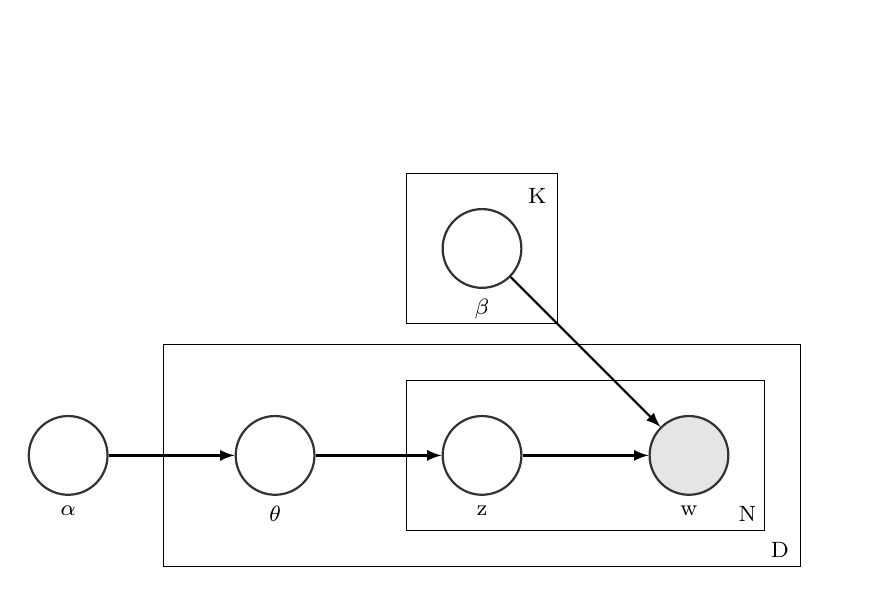
\begin{tikzpicture}
\tikzstyle{main}=[circle, minimum size = 10mm, thick, draw =black!80, node distance = 16mm]
\tikzstyle{connect}=[-latex, thick]
\tikzstyle{box}=[rectangle, draw=black!100]
  % sigma
  \node[main] (alpha) [label=below:$\alpha$] { };    
  % eta
  \node[main] (theta) [right=of alpha,label=below:$\theta$] { };
  % z
  \node[main] (z) [right=of theta,label=below:z] {};
  % beta
  \node[main] (beta) [above=of z,label=below:$\beta$] { };
%  \node[main] (beta) [left=of psi,label=below:$\beta$] { };
  \node[main, fill = black!10] (w) [right=of z,label=below:w] { };
  \path (alpha) edge [connect] (theta)
        (theta) edge [connect] (z)
		(z) edge [connect] (w)
		(beta) edge [connect] (w);
%		(beta) edge [connect] (psi);
  \node[rectangle, inner sep=4.4mm,draw=black!100, fit= (beta)] {};
  \node[rectangle, inner sep=4.4mm, fit= (beta), label=below right:K, xshift=-5mm, yshift=18.5mm] {};
  \node[rectangle, inner sep=0mm, fit= (z) (w),label=below right:N, , xshift=13mm] {};
  \node[rectangle, inner sep=4.4mm,draw=black!100, fit= (z) (w)] {};
    \node[rectangle, inner sep=4.6mm, fit= (z) (w),label=below right:D, xshift=12.5mm] {};
  \node[rectangle, inner sep=9mm, draw=black!100, fit = (theta) (z) (w)] {};
\end{tikzpicture}
\caption{Graphical representation for CTM}
\label{graph:ctm}
\end{figure}
\begin{algorithm}[H]
Initialize $ \mu, \Sigma $\\
\For{document d in D}{
Sample a topic distribution $ \eta_d\sim\mathcal{N}(\mu,\Sigma) $\\
\For{word position n in $ N_d $}{
Sample a topic assignment $ z_{dn}\sim \text{Mult}(f(\eta_d)) $\\
Sample a word $ w_{dn}\sim \text{Mult}(\beta_{z_d,n}) $
}
}
\label{algorithm:ctm}
\caption{Generative Process for CTM}
\end{algorithm}
From Algorithm \ref{algorithm:ctm}, the parametrization $ \mu, \Sigma $ are initialized. For each document d in document collection D, a topic distribution $ \eta_d $ is drawn from normal distribution parametrized $ \mu,\Sigma $. Then for each word position n in $ N $ words in doucment d, a topic assignment $ z_{dn} $ is drawn from multinomial distribution parametrized $ f(\eta_d) $, where the transformation $ f(\eta) $ represents the softmax function maps the sample draw from normal distribution to topic proportion $ \theta $, a topic distribution which points on the K-1 simplex. Finally, a word is sampled from multinomial distribution $ Mult(\beta_{z_d,n}) $.

From figure \ref{graph:ctm} we can see, word and topic-word assignment are in the word and document plate $ N\times D $. The document topic proportion $ \eta $ is on the document plate D. Specifically, the topic word proportion $ \beta $ is on the topic plate K, which is specified as word distribution selected by topic assignment z. 

\paragraph{Mathematical Formulation} The joint distribution for CTM is described as follows,
\begin{align*}
p(\eta,z,w|\beta,\mu,\Sigma)=\prod_{d=1}^{D}p(\eta_d|\mu,\Sigma)\prod_{n=1}^{N_d}p(z_{dn}|\eta_d)p(w_{dn}|z_{dn},\beta_{1:K})
\end{align*}
and the ELBO is defined as,
\begin{align*}
\mathcal{L}\geq&\sum_{d=1}^{D}\mathbb{E}_{q_d}\left[\log p(\eta_d,z_d,w_d|\mu,\Sigma,\beta_{1:K})\right]-\sum_{i=1}^{K}\log\text{KL}(q(\eta_i|\lambda_i,\nu_i^2)|p(\eta_d|\mu,\Sigma))\\
&-\sum_{n=1}^{N}\log\text{KL}(q(z_n|\phi_n)||p(z_n|\eta_d))
\end{align*}
\section{LKJ Correlation Distribution} \label{ch2:lkj}
LKJ distribution \cite{lewandowski_generating_2009} is a distribution for modeling correlation matrix. The distribution is described as equation \ref{eq:lkj}
\begin{align} \label{eq:lkj}
f(C|\eta)=&2^{\sum_{k=1}^{K-1}(2(\eta-1)+K-k)(K-k)}\times\\
&\prod_{k=1}^{K-1}(B(\eta+(K-k-1)/2,\eta+(K-k-1)/2)^{K-k})(\det(C)^{\eta-1})
\end{align}
When $ \eta=1 $ it is simply a uniform distribution allocated over the correlation matrix. If $ \eta>0 $, it is a modal correlation matrix. The density concentrated around center when the $ \eta $ value become larger.
To apply it into normal distribution as covariance, we could apply transformation equation \ref{eq:lkj_trans} and turn it into covariance matrix\cite{barnard_modeling_2000}.
\begin{align}\label{eq:lkj_trans}
\Sigma=diag(\sigma)\cdot C \cdot diag(\sigma)
\end{align}
% Transformation
Directly drawing correlation matrix from LKJ distribution is not practical in reality case. It is common to draw correlation matrix from factorized Cholesky LKJ distribution instead, where the probability density function is described as equation \ref{eq:lkj_chol}
\begin{align} \label{eq:lkj_chol}
\text{LKJChol}(L|\eta)&\propto|J|\det(LL^\top)^{(\eta-1)}\\
&=\prod_{k=2}^{K}L_{kk}^{K-k+2\eta-2}
\end{align}
The lower triangular matrix L is a Cholesky factorization for the correlation matrix iff $ L_{k,k}>0 $
\begin{align}
\Sigma=\text{diag}(\sigma)\cdot LL^\top \cdot \text{diag}(\sigma)
\end{align}
similarly, the transformation from LKJ Cholesky matrix to covariance matrix as equation \ref{eq:lkj_trans}.
\section{Embedded Topic Model} \label{ch2:etm}
Embedded Topic Model \cite{dieng_topic_2019} is one of the state-of-art approaches for topic model task. It takes word distribution $ \beta $ as a topic embedding for words. % explain the algorithm
Similar to Word2Vec\cite{mikolov_distributed_nodate}, the word distribution is a softmax function of the inner product of context matrix $ \rho $ and context embedding $ \alpha $. Specifically, the algorithm   equation \ref{eq:etm_embedding}
\begin{equation}\label{eq:etm_embedding}
\beta\sim\sigma(\rho^\top\alpha)
\end{equation}
The word is drawn from the generative process shown in algorithm \ref{algorithm:etm}, for each document, sample a topic distribution $ \theta $ from logistic-normal distribution parameterized with zero mean and identity covariance. Then for each word position n, the model sample topic assignment $ z_{dn} $ from categorical distribution $ \theta_d $. Finally, a word is drawn from $ \text{softmax}(\rho^\top\alpha) $ on $ z_{dn} $ the row.\\
\begin{algorithm}[H]\label{algorithm:etm}
\ForEach{document $d\in 1\dots D $}{
Draw document topic distribution $ \theta_d\sim \mathcal{LN}(0,I) $\\
\ForEach{word position $n\in 1\dots N_d $}{
%Generate topic $ z_{d,n}\sim Cat(\eta_d) $\\
Draw topic assignment $ z_{d,n}\sim Cat(\theta_d) $\\
Draw word $ w_{d,n}\sim \sigma(\rho^\top\alpha)_{z_{dn}} $
}}
\caption{Generative Process for ETM}
\end{algorithm}
Although ETM can maintain for Word2Vec training as the embedding for topic modeling, it cannot capture 
\section{Transformer} \label{ch2:transformer}
Transformer\cite{vaswani_attention_nodate} is a popular neural network architecture in natural language processing. To briefly explain Transformer, it is an stacked encoder-decoder architecture. The component that makes transformer stands out of other architectures it the attention mechanism. The attention mechanism 
\chapter{Topic Model with Transformer Embeddings}\label{ch3}
In this chapter, we give a detailed explanation and procedure of LKJTM to be implemented.
\section{Correlated Topic Model with Transformer Embeddings}
The TETM utilizes the Transformer as embedding to the topic-word representations. To compare with the original topic model, the word-topic distribution $ \beta $ is the 
First, the topic embedding embeds the vocabulary into L-dimensional space, which is by Transformer embedding. Second, the context embedding maps the embedding into K-dimensional space . 
In the generative process, the LKJTM uses the topic embedding to form a per-topic vector to represent the meaning over the vocabulary. 
% LKJ Prior
\section{LKJ correlation prior}
\begin{algorithm}[H]
Initialize hyperparameters $ \gamma $, $ \mu $\\
Sample Correlation Matrix $ L\sim \text{LKJChol}(\gamma)$\\
\For{document d in D}{
Sample topic distribution $ \theta_d\sim \mathcal{LN}(\mu,\sigma LL^\top\sigma) $\\
\For{word position n in $ N_d $}{
Sample word $ w_{d,n}\sim \sigma(\theta_d(\rho^\top\alpha)_{\cdot,w_{d,n}}) $
}
}
\caption{Generative Process for LKJ correlation prior}
\label{algorithm:lkjtm}
\end{algorithm}
% Graphical Model'
\begin{figure}
\centering
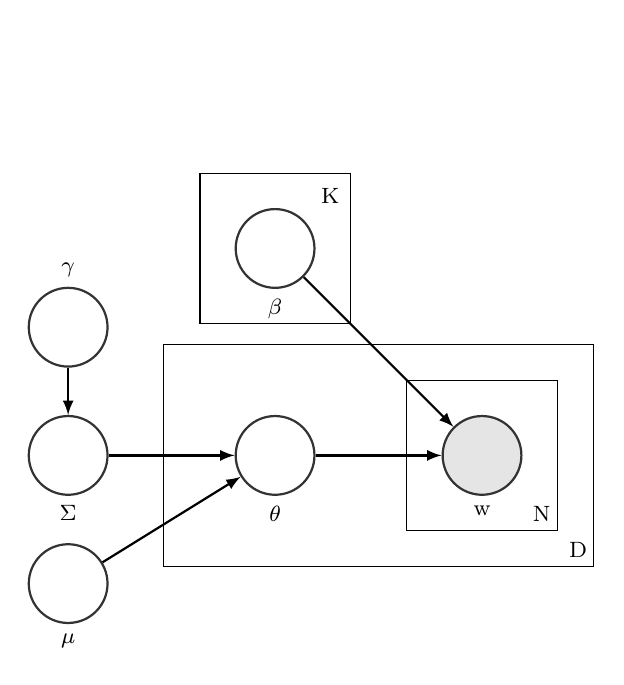
\begin{tikzpicture}
\tikzstyle{main}=[circle, minimum size = 10mm, thick, draw =black!80, node distance = 16mm]
\tikzstyle{connect}=[-latex, thick]
\tikzstyle{box}=[rectangle, draw=black!100]
  % sigma
  \node[main] (sigma) [label=below:$\Sigma$] { };    
  % mu
  \node[main] (mu) [yshift=1cm, below=of sigma, label=below:$\mu$] { };
  % gamma
  \node[main] (gamma) [yshift=-1cm, above=of sigma, label=above:$\gamma$] { };
  % eta
  \node[main] (theta) [right=of sigma,label=below:$\theta$] { };
  % z
%  \node[main] (z) [right=of theta,label=below:z] {};
  % beta
  \node[main] (beta) [above=of theta,label=below:$\beta$] { };
%  \node[main] (beta) [left=of psi,label=below:$\beta$] { };
  \node[main, fill = black!10] (w) [right=of theta,label=below:w] { };
  \path (gamma) edge [connect] (sigma)
  		(sigma) edge [connect] (theta)
  		(mu) edge [connect] (theta)
        (theta) edge [connect] (w)
%		(z) edge [connect] (w)
		(beta) edge [connect] (w);
%		(beta) edge [connect] (psi);
  \node[rectangle, inner sep=4.4mm,draw=black!100, fit= (beta)] {};
  \node[rectangle, inner sep=4.4mm, fit= (beta), label=below right:K, xshift=-5mm, yshift=18.5mm] {};
  \node[rectangle, inner sep=0mm, fit= (w),label=below right:N, , xshift=0mm] {};
  \node[rectangle, inner sep=4.4mm,draw=black!100, fit=  (w)] {};
  \node[rectangle, inner sep=4.6mm, fit= (w),label=below right:D, xshift=0mm] {};
  \node[rectangle, inner sep=9mm, draw=black!100, fit = (theta) (w)] {};
\end{tikzpicture}
\caption{Graphical model for LKJTM}
\label{graph:lkjtm}
\end{figure}

% Generative process
The generative process of the $ d^{th} $ document is the following:\\
\begin{algorithm}[H]
Initialize hyperparameters $ \gamma $, $ \mu $\\
Sample Correlation Matrix $ L\sim \text{LKJChol}(\gamma)$\\
\For{document d in D}{
Sample topic distribution $ \theta_d\sim \mathcal{LN}(\mu,\sigma LL^\top\sigma) $\\
\For{word position n in $ N_d $}{
Sample word $ w_{d,n}\sim \sigma(\theta_d(\rho^\top\alpha)_{\cdot,w_{d,n}}) $
}
}
\caption{Generative Process for LKJTM}
\label{algorithm:lkjtm}
\end{algorithm}
From algorithm \ref{algorithm:lkjtm}, starting from step 1, the topic proportion $ \theta_d $ is drawn from the logistic-normal distribution $ \mathcal{LN}(\cdot) $ with zero mean and identical covariance.
From Step 2-a, for each word position $ n $ in document $ d $, a topic assignment to word $ w_{dn} $ is drawn from categorical distribution $ Cat(\theta_d) $ parameterized by topic proportion $ \theta_d $
Step 2-b, the model draw a word from embedding of the vocabulary $ \rho $ and the assigned topic embedding $ \alpha_{z_{dn}} $ to draw the observed word from the assigned topic, as given by $ z_{dn} $. The embedding is applied softmax function to make them topic distribution.
The TETM likelihood uses a matrix of word embedding $ \rho $, a representation of the vocabulary in a lower dimensional space. In practice, it can either rely on previously fitted embeddings as part of the fitting procedure, it simultaneously finds topics and an embedding space.

% TODO LKJ Correlation Distribution Formulation

% TODO Transformer Embeddings
% Transformer embeddings
\section{Transformer Embeddings}
Following the ETM architecture, we modify topic-word distribution as an embedding and put transformer embedding to work into it. 
\begin{equation}\label{eq:transformer_embedding}
\beta\sim\text{softmax}(\rho^\top\alpha)
\end{equation}
Equation \ref{eq:transformer_embedding}, 
% Marginal Likelihood
\section{Marginal Likelihood}
The parameter $ \alpha $ is the topic embedding on the word embedding space of dimension K. We take a log marginal likelihood of the document,
\begin{align*}
\mathcal{L}(\alpha)=\sum_{d=1}^{D}\log p(w_d|\alpha)
\end{align*}
\begin{align*}
p(w_d|\alpha)=\int p(\theta_d|\mu,\Sigma)\prod_{n=1}^{N_d}p(w_{dn}|\theta_d,\alpha)d\theta_d
\end{align*}
the conditional distribution $ p(w_{dn}|\theta_d,\alpha) $ marginalize out the the topic assignment $ z_{dn} $,
\begin{align*}
p(w_{dn}|\theta_d,\alpha)=\sum_{k=1}^{K}\theta_{dk}\beta_{k,w_{dn}}
\end{align*}
where $ \beta $ represent the topic-word distribution, composed of transformer embedding $ \rho $ and topic embedding $ \alpha $, in such case
\begin{align*}
\beta_{kv}=\text{softmax}(\rho^\top\alpha)_{v}.
\end{align*}
then we take the amortized inference to take out neural network for the representation,
\begin{align*}
p(w_{d}|N(\mu_\theta(w),\sigma_\theta(w)),\beta)=\mathbb{E}_{\theta\sim N(\mu_\theta(w),\sigma_\theta(w))}\left[w^\top\sigma(\beta\theta)\right]
\end{align*}
Reparametrization Trick $ \theta=\mu+\sigma^{1/2}\epsilon $\\
\begin{align*}
p(w_{d}|\mu_\theta(w)+\epsilon\sigma^{1/2}_\theta(w),\beta)=\mathbb{E}_{\epsilon\sim N(0,1)}\left[w_d^\top\sigma(\beta(\mu_\theta(w)+\epsilon\sigma^{1/2}_\theta(w)))\right]
\end{align*}
%% Joint Distribution
\section{Joint Distribution}
We give a description of the joint distribution, $ W,Z,\theta $ and $ \Sigma $ are variables and $ \beta, \mu $ and $ \gamma $ are latent variables. $ W $ is the word likelihood from the document collections, $ Z $ represents the topic-word assignment, $ \theta $ models the topic distribution for each document, and $ \Sigma $ is the covariance matrix which depends on the document-topic distribution $ \theta $.
\begin{align*}
p(W,Z,\theta,\Sigma|\beta,\mu,\gamma)&=P(W|Z)P(Z|\theta)P(\theta|\mu,\Sigma)\\
&=p(\Sigma|\gamma)\prod_{d=1}^{D}P(\theta_d|\mu,\Sigma)\prod_{n=1}^{V}P(z_{d,n}|\theta_d)P(w_{d,n}|z_{d,n},\beta)
\end{align*}
by taking  log on the joint probability, we obtain a objective function for optimization
\begin{align*}
\log p(W,Z,\theta,\Sigma|\beta,\mu,\gamma)=&\sum_{d=1}^{D}\left[\log P(\theta_d|\mu,\Sigma)+\sum_{n=1}^{V}\left[\log P(z_{d,n}|\theta_d)+\log P(w_{d,n}|z_{d,n},\beta)\right]\right]\\
&+\log p(\Sigma|\gamma)
\end{align*}
\section{Inference and Estimation}
% Inference Equation
% Variational Inference
% KL-divergence for the logistic normal distribution
\subsection{Evidence Lower Bound(ELBO)}\label{ch3:2} To perform Variational inference, it is essential to derive the Evidence Lower Bound (ELBO) first as the objective function for the optimization. By equation \ref{eq:ch3_elbo1}
\begin{align}\label{eq:ch3_elbo1}
\mathcal{L}(\alpha,\rho,\nu)=\sum_{d=1}^{D}\sum_{n=1}^{N_d}\mathbb{E}_q[\log p(w_{dn}|\theta_d,\rho,\alpha)]-\sum_{d=1}^{D}KL(q(\theta_d|w_d,\nu)||p(\theta_d))
\end{align}
% TODO Monte Carlo Estimate
\paragraph{Monte-Carlo estimation}
The expectation log likelihood term in \ref{eq:ch3_elbo2} can be efficiently approximated by the Monte Carlo sampling method,
\begin{align}\label{eq:ch3_elbo2}
\mathcal{L}\approx\frac{1}{S}\sum_{s=1}^{S}\sum_{d=1}^{D}\sum_{n=1}^{N_d}\mathbb{E}_q[\log p(w_{dn}|\theta_d^{(s)},\rho,\alpha)]-\sum_{d=1}^{D}KL(q(\theta_d|w_d,\nu)||p(\theta_d))
\end{align}
Here we define amortized inference, a optimization technique which perform inference by defined neural networks. $ \mu_\theta(w) $ and $ \sigma_\theta(w) $ are two inference networks take input from the word $ w $. Then a output is generated by the Normal distribution parameterized by $ \mu_\theta(w) $ and $ \sigma_\theta(w) $.
\begin{align}\label{eq:ch3_elbo3}
=&\sum_{d=1}^{D}\left(\mathbb{E}_{q(\theta_d)}\left[\log p(w_d|\mathcal{LN}(\mu_{\theta_d}(w_d),\sigma_{\theta_d}(w_d)),\beta)\right]-KL(q(\theta_d|w_d,\nu)||p(\theta_d))\right)
\end{align}
To apply reparameterization trick, we take transformation from normal distribution to $ \theta=\mu+\epsilon\sigma^{1/2} $ where $ \epsilon\sim N(0,1) $, as  equation \ref{eq:elbo_5}
\begin{align}\label{eq:elbo_5}
=&\sum_{d=1}^{D}\left(\mathbb{E}_{q(\epsilon)}\left[\log p(w_d|\sigma(\mu_{\theta_d}(w_d)+\epsilon\sigma_{\theta_d}(w_d)),\beta)\right]-KL(q(\theta_d|w_d,\nu)||p(\theta_d))\right)
\end{align}
we also apply the mini-batch to make able the model perform by sub-sampling the document collection. By equation \ref{eq:elbo_6}
\begin{align}\label{eq:elbo_6}
\tilde{\mathcal{L}}=&\frac{\mathcal{D}}{|\mathcal{B}|}\sum_{d\in\mathcal{D_B}}\left(\mathbb{E}_{q(\epsilon)}\left[\log p(w_d|\sigma(\mu_{\theta_d}(w_d)+\epsilon\sigma_{\theta_d}(w_d)),\beta)\right]-KL(q(\theta_d|w_d,\nu)||p(\theta_d))\right)
\end{align}
The KL-divergence for the logistic-normal distribution is given as equation \ref{eq:elbo_7} closed-form expression,
\begin{align}\label{eq:elbo_7}
\text{KL}(q(\theta_d)||p(\theta_d))=-\frac{1}{2}\left(tr(\sigma_1^{-1}\sigma_0)+(\mu_1-\mu_0)\Sigma_1^{-1}(\mu_1-\mu_0)-K+\log\frac{|\sigma_1|}{|\sigma_0|}\right)
\end{align}
we plug in the likelihood term from equation \ref{eq:placeholder}, thus the ELBO then becomes \ref{eq:elbo_8}
\begin{align}\label{eq:elbo_8}
\tilde{\mathcal{L}}=&\sum_{d=1}^{D}\left[-\frac{1}{2}\left(tr(\sigma_1^{-1}\sigma_0)+(\mu_1-\mu_0)\Sigma_1^{-1}(\mu_1-\mu_0)-K+\log\frac{|\sigma_1|}{|\sigma_0|}\right)\right]\\
&+\mathbb{E}_{\epsilon\sim\mathcal{N}(0,I)}\left[w_d^\top\log\sigma(\beta(\mu_0+\sigma_0^{1/2}\epsilon))\right]
\end{align}
% TODO Transformer Loss
\subsection{Transformer Loss}
It is suggested that using cross entropy loss for transformer training. In equation \ref{eq:crossentropy}, . It is worth mention that, the 
\begin{align}\label{eq:crossentropy}
L_{\text{CrossEntropy}}=-\frac{1}{V}\sum_{i=1}^{V}y_i\cdot\log(\hat{y_i})
\end{align}
% TODO algorithm for the optimization here
\subsection{Optimization step}\label{ch4:3}
In algorithm \ref{algorithm:lkjtm_obj}, first initialize the model and variational parameters. Then, for each epochs, we obtain the transformer embedding $ \rho $ from transformer. After that, the topic embedding $ \beta $ is computed by taking softmax of dot-product of $ \rho $ and $ \alpha $. Then a minibatch $ \mathcal{B} $ is selected from the document for optimization. The number of minibatch is the document collection divides minibatch size where $ \#\text{minibatch}=\frac{\mathcal{D}}{|\mathcal{B}|} $. For each minibatch, the model takes a document and sample lower Cholesky matrix from LKJ Cholesky distribution(description see section \ref{ch2:lkj}). A topic assignment for document d $ \theta_d $ is sampled from logistic-normal distribution $ \mathcal{LN}(\mu,\sigma LL^\top\sigma) $, where $ \mu $ is sampled from half-Cauchy distribution and covariance is a transformation from equation \ref{eq:lkj_trans}. For each word position n, a word is sampled from the softmax of dot-product of transformer embedding $ \rho $ and NN weight $ \alpha $. After the sampling process for the document collection, we estimate the ELBO loss $ L_{ELBO} $ for the topic model, and the cross entropy loss $ L_{CrossEntropy} $. Remind that the topic model and transformer take input differently. The topic model part takes bag-of-words input, a document-vocabulary matrix $ D\times V $ counting the occurrence of vocabulary v in document d. While transformer take sequence of document as input. 
To calculate the loss of the model , we sum up the ELBO loss $ L_{ELBO} $ and cross entropy loss for transformer $ L_{CrossEntropy} $. Then a stochastic gradient is computed by backpropagation. a gradient step to . The process iterates until the maximum iteration is reached. 
\\
\begin{algorithm}[H]
Initialize model and variational parameters\\
\For{epoch $i=1,2,\dots N$}{
Compute the trnasformer embedding $ \rho $\\
Compute $ \beta=\text{softmax}(\rho^\top\alpha) $\\
Choose a minibatch $ \mathcal{B} $ of documents\\
\ForEach{document d in $ \mathcal{B} $}{
Compute $ \mu_d=\text{NN}(x_d;\nu_\mu) $\\
Compute $ \sigma_d=\text{NN}(x_d;\mu_\sigma) $\\
Sample $\theta_d\sim\mathcal{LN}(0,I_k)$\\
\ForEach{word position n in docuemnt $ N_d $}{
Sample word $ w_{dn}\sim \text{softmax}(\beta_{w_{dn}}\theta_{d}) $
}
}
Estimate ELBO loss $ \text{L}_\text{ELBO}$ from Eq. \ref{eq:elbo_8}\\
Compute Transformer loss $ \text{L}_\text{CrossEntropy}$ from Eq. \ref{eq:crossentropy}\\
Compute the total loss $ \text{L}=\text{L}_\text{ELBO}+\text{L}_\text{CrossEntropy} $\\
Compute the stochastic gradient via backpropagation\\
Take a stochastic gradient step\\
Update model parameters ($\rho,\alpha,$)\\
Update variational parameters ($ \ $)
}
\label{algorithm:lkjtm_obj}
\caption{Topic modeling with the LKJTM}
\end{algorithm}
%\begin{algorithm}[H]
%Initial $ \theta^{(0)} $ randomly\\
%\While{Not Converge}{
%Sample a document d uniformly from dataset $ \mathcal{D} $\\
%For all k, initial $ \gamma^{d}_{k}=1 $\\
%\While{Not Converge}{
%\For{$ i=1,\cdots,N_d $}{
%\begin{align*}
%\phi_{ik}^{d}\propto\exp{\mathbb{E}}[\log\pi^d_k]+\mathbb{E}[\log\beta_{k,w_i^d}]
%\end{align*}
%}
%Set $ \gamma^{d}=\alpha+\sum_{i=1}^{N_d}\phi_i^d $
%}
%Take a stochastic gradient step $ \theta^{t}=\theta^{t-1}+\epsilon_t+\triangledown_\theta\mathcal{L}_d $
%}
%\caption{SVI for LDA}
%\end{algorithm}
\section{Results \& Evaluations}
In this chapter, we perform evaluation on our model and the other algorithms, the repository of our model is provided in github \footnote{\url{https://github.com/cwleung/LKJTM}}.
\subsection{Experiment Testing}
The experiment will be conducted with a number of existing proposed topic models as mentioned related work section above. We conduct the experiment with those baseline algorithms and evaluate them in terms of accuracy and running time. Some of the source code of competitive were provided by their authors in Github\footnote{For instance, Correlated Topic Model(CTM), \href{https://github.com/blei-lab/ctm-c}{https://github.com/blei-lab/ctm-c}}. The outcome result will be extensively studied and conclude the insight behind the algorithms and methodologies. Detail to be stated in section \ref{AD}. Our probabilistic part of model implemented using Pyro\cite{bingham_pyro_2019}, while the model optimization and transformer implementations are based on PyTorch\cite{paszke_automatic_2017}.
\subsection{Dataset}To evaluate the performance of the model, we select the two most poplar data set in the context of topic model evaluation. 20Newsgroups and Reuter RCV1-v2 datasets. 20NewsGroup consist of 18,846 news group documents \footnote{\url{http://qwone.com/~jason/20Newsgroups/}} and the RCV1-v2 includes 10,000 documents in total. Both of the dataset will be preprocessed to remove stopwords and stemming before the evaluation. If desirable, it will also to be applied to NIST TREC dataset and NII NTCIR dateset for further application studies.
\subsection{Data Preprocessing}
We perform data preprocessing, tokenization, stopword removal, lemmatization, and set the 
\subsection{Models}
We compare the model performance with a numbers of rivals. We take Latent Dirichlet Allocation (LDA)\cite{blei_latent_2003} as the baseline model. Other models include Transformer\cite{vaswani_attention_nodate}\footnote{Not a topic model, but we think it is worth to make comparison still.},  ProdLDA\cite{srivastava_autoencoding_2017} and Embedded Topic Model(ETM)\cite{dieng_topic_2019}.
\subsection{Algorithmic Settings}
% optimization algorithm
To perform posterior inference, we employed Stochastic Variational Inference (SVI) \cite{hoffman_stochastic_2013} for the optimization problem. We set the minibatch size to 1024 documents.
% Other model
For LDA, we applied the model provided from sklearn package (version 0.24.0) \footnote{Sklearn website \url{https://scikit-learn.org/stable/index.html}}. For ETM, we run the experiment with the parameter suggested \cite{dieng_topic_2019}. For ProdLDA, we perform optimization with inference network architecture as described in the paper \cite{srivastava_autoencoding_2017}. 
% learning rate
To perform optimization, we use Adam for the gradient ascent algorithm, and we set the learning rate to 1e-3.
% l2-regularization factor
we use $ l2 $-regularization to the 
% inference network [size, activation function, dropout, batch-norm]
We use 
% Transformer settings

% 
\subsection{Quantitative Result}
In this section, we evaluate the model with the following metric adopted from \cite{dieng_dynamic_2019}: Perplexity, Topic Coherence (TC), Topic Diversity (TD). %and Topic Quality (TQ).\begin{center}
\begin{table}[h]
\centering
\begin{tabular}{llll}
\hline
Model      & TC     & Perplexity  \\ \hline
Transformer & -0.311 & - \\
LDA & 0.183 & 2425.9 \\
ProdLDA		&  0.107 & 5652.0\\
ETM	     	&  0.177 & \textbf{1919.3}\\
\textbf{Our model}  & \textbf{0.206} & 3444.1 \\ \hline
\end{tabular}
\label{tbl:t1}
\caption{Result of our implementation(topic k=20)}
\end{table}
\begin{table}[h]
\centering
\begin{tabular}{llll}
\hline
Model      & TC     & Perplexity  \\ \hline
Transformer & -0.251 & - \\
LDA & 0.155 & \textbf{2536.1} \\
ProdLDA		&  0.074 & 5654.1\\
ETM	     	&  0.145 & 2603.9\\
\textbf{Our model}  & \textbf{0.199} & 3705.0 \\ \hline
\end{tabular}
\label{tbl:t2}
\caption{Result of our implementation(topic k=50)}
\end{table}
\paragraph{Discussion}On the result from table \ref{fig:eval_20ng_20t}, \ref{fig:eval_20ng_50t}, display that our model has outperform the other model by TC score. On perplexity score, ETM obtain the best score when $ k=20 $ and LDA when $ k=50 $. Since Transformer is not a topic model actually, it got a negative score on TC, which refers it cannot retrieve any useful topic from documents.
\subsection{Training}
From figure \ref{fig:loss_20ng_20t}, \ref{fig:loss_20ng_50t}, display the training process of the training loss and log probability by 200 epochs. From \ref{fig:eval_20ng_20t}, \ref{fig:eval_20ng_50t}, we observe that the TD score and TC score increase monotonically, however, the perplexity increases throughout the epochs. 
\subsection{Qualitative Result}The proposed model will be evaluated with a number of specifically selected topic and examined with their performance separately. The result will be exhaustively compared with other existing models.\\
From table \ref{tbl:t3}, we have selected some topic words each model generated from 20Newsgroups when $ k=20 $. The topics represent space, operating system, religion, encryption and guns respectively. Our model has shown capability on capturing key words from each topic, such as on topic "space": \textit{nasa}, \textit{space}, \textit{jpl}, \textit{moon}, \textit{earth}, \textit{station}, \textit{flight} are the outputs.
\begin{table}[h]
\centering
\begin{tabular}{llll}
\hline
Our Model  \\ \hline
\textbf{nasa }gov \textbf{space jpl moon earth station flight }research digex\\
\textbf{windows window }problem \textbf{dos }running \textbf{file mouse }mit de ms\\
\textbf{god jesus christian }people faith bible time church good things\\
key chip encryption clipper security privacy government keys public escrow\\
gun people control government guns weapons american make clinton state \\ \hline
\hline
ProdLDA  \\ \hline
nasa space gov people station time orbit dc program shuttle \\
scsi drive controller max drives ide senior tape time people \\
god jesus atheists christian bible religion atheism christians word truth \\
key crypto session nt chips chip serial dos keys encrypted \\
gun people god religion writes life morality ohio argument question \\ \hline
\hline
LDA  \\ \hline
space, nasa, gov, access, launch, earth, digex, moon, orbit\\
file, window, program, ftp, files, server, image, graphics, windows\\
god, people, jesus, christian, bible, writes, life, christians, time\\
key, encryption, chip, clipper, keys, security, government, privacy\\
gun, guns, law, police, people, weapons, crime, fbi, control
\\ \hline
\hline
ETM  \\ \hline
space, nasa, gov, mr, president, health, research, year, center\\
windows, file, window, program, files, server, version, dos, image\\
god, people, jesus, christian, israel, bible, jews, christians, israeli\\
key, encryption, chip, clipper, keys, privacy, security, technology, government\\
gun, people, government, law, state, guns, article, weapons, control
\\ \hline
\end{tabular}
\label{tbl:t3}
\caption{Top-9 words for each topic from randomly selected 5 topics}
\end{table}
\begin{figure}[h]
\centering
\subcaptionbox{Log probability}{\includegraphics[width=0.50\textwidth]{figure/0908/log_prob_20t}}%
\hfill
\subcaptionbox{Negative ELBO}{\includegraphics[width=0.50\textwidth]{figure/0908/elbo_20t}}%
\hfill
\caption{20Newsgroups (k=20)}
\label{fig:loss_20ng_20t}
\end{figure}
\begin{figure}
\centering
\subcaptionbox{Log probability}{\includegraphics[width=0.50\textwidth]{figure/0908/log_prob_50t}}%
\hfill
\subcaptionbox{Negative ELBO}{\includegraphics[width=0.50\textwidth]{figure/0908/elbo_50t}}%
\hfill
\caption{20Newsgroups (k=50)}
\label{fig:loss_20ng_50t}
\end{figure}
\begin{figure}
\centering
\subcaptionbox{Topic Diversity}{\includegraphics[width=0.50\textwidth]{figure/0908/td_20t}}%
\hfill
\subcaptionbox{Topic Coherence}{\includegraphics[width=0.50\textwidth]{figure/0908/tc_20t}}%
\hfill
\subcaptionbox{Perplexity}{\includegraphics[width=0.50\textwidth]{figure/0908/ppl_20t}}%
\hfill
\caption{20Newsgroups (k=20)}
\label{fig:eval_20ng_20t}
\end{figure}
\begin{figure}
\centering
\subcaptionbox{Topic Diversity}{\includegraphics[width=0.50\textwidth]{figure/0908/td_50t}}%
\hfill
\subcaptionbox{Topic Coherence}{\includegraphics[width=0.50\textwidth]{figure/0908/tc_50t}}%
\hfill
\subcaptionbox{Perplexity}{\includegraphics[width=0.50\textwidth]{figure/0908/ppl_50t}}%
\hfill
\caption{20Newsgroups (k=50)}
\label{fig:eval_20ng_50t}
\end{figure}
\subsection{Visualization}
To clearly demonstrate the representation for , we applied t-SNE to map the topic-word representation into 2-dimension continuous space. In figure \ref{fig:tsne20t25w2} and \ref{fig:tsne50t25w0}, demonstrate the t-SNE visualization of the topic-word distribution for 20Newsgroups. 
\begin{figure}
\centering
\includegraphics[width=1\linewidth]{figure/0908/tsne_20t_25w_2}
\caption{Visualization \#Topics:20}
\label{fig:tsne20t25w2}
\end{figure}
\begin{figure}
\centering
\includegraphics[width=1\linewidth]{figure/0908/tsne_50t_25w_0}
\caption{Visualization \#Topics:50}
\label{fig:tsne50t25w0}
\end{figure}

\chapter{LKJ Prior Correlated Topic Model with Transformer Embeddings}\label{ch4}
In this chapter, we give a detailed explanation and procedure of Transformer embedding with Correlated Topic Model(TECTM) to be implemented.
\section{Introduction}
\paragraph{}Latent dirichlet allocation(LDA)\cite{blei_latent_2003} is one of the popular model in topic modeling. However, the model take bag-of-word assumption that all words are independently distributed. Also, the original model take optimization step on entire set of document, where it limits the size of the data set can be trained within a limited memory size and hence scalability is a concern for LDA.
% Correlated Topic Model
Correlated Topic Model(CTM)\cite{blei_correlated_2007} take consideration between topics by implementing the correlation information over the document-topic proportion. However, the model does not make assumption of prior information on the covariance matrix.
% Embedded Topic Model
Embedded Topic Model(ETM)\cite{dieng_topic_2019} explore the possibilities the word2vec embedding to be working together with topic model to improve the quality of topic-words generation. However, since word2vec is a simple embedding architecture, the model could be better to be working with embedding that captures positional information.
% Intro
\paragraph{}In this chapter, we propose Transformer embedding with Correlated Topic Model(TECTM), a topic model that takes prior assumption on covariance matrix over the document-topic distribution, and integrate Transformer with the topic model to maintain a better quality of word representations in latent space.
% LKJ Prior
We propose LKJ correlation prior into our correlated topic model, where the correlation prior take place to capture correlation between topics by modeling the proportion over document-topic.
% Positional information
To take advantage of positional information, we access the possibility the use of Transformer model to improve topic model performance. Transformer takes input sequence from documents and perform scaled dot-product to compute the each token in a sentence relates each other and the importance over a hidden context.
% topic model
In the following of the chapter, we first go through the related works that have been proposed by other authors. Then, we define the proposed model TECTM and derive its inference process. After that, we explain the implementation detail and the algorithmic setting for the experiment. Finally, the results are compared with other state-of-the-art models and discuss the performance our model out perform the other instances.
\section{Related works}
Correlated Topic Model (CTM)\cite{blei_correlated_2007} is the original work that proposed to alleviate the problem LDA, which did not utilize the topic information between correlated topics. The proposed model replaced Dirichlet distribution with a logistic-normal prior with covariance matrix to represent the relationship between topics.

There have been a several of works focus on word embedding and topic model. Major of them combined statistical model and embedding approach to model topic distribution. In other words, these method representing a word by mapping every single word into continuous space instead of using a probability distribution as was in typical LDA model.
%% Embedded Topic Models
Embedded Topic Model\cite{dieng_topic_2019} uses word2vec embedding to capture the word representation in latent continuous space. The posterior of the model was approximated by amortized inference.
% # CGTM
Xun \cite{xun_correlated_2017} employed words embedding into Correlated Topic Model, the new correlated topic model as Correlated Gaussian Topic Model (CGTM). In their paper they make use of word embedding space and model the correlation between topics by calculation of similarity between words in the embedding space.
% # CTMTE
Similarly, He\cite{he_efficient_2017} proposed Correlated Topic Modeling with Topic Embedding (CTMTE), which transformed the topic distribution previously obtained into lower dimension topic embedding space. The correlation between topics were directly computed through the similarity calculation in the vector space. The paper stated it reduces the running time as a scalable framework into large applications.
\section{Model description}
The TECTM utilizes the Transformer as embedding to the topic-word representations. To compare with the original topic model, the word-topic distribution $ \beta $ is the 
First, the topic embedding embeds the vocabulary into L-dimensional space, which is by Transformer embedding. Second, the context embedding maps the embedding into K-dimensional space . 
In the generative process, the TECTM uses the topic embedding to form a per-topic vector to represent the meaning over the vocabulary. 
% Graphical Model'
\begin{figure}
\centering
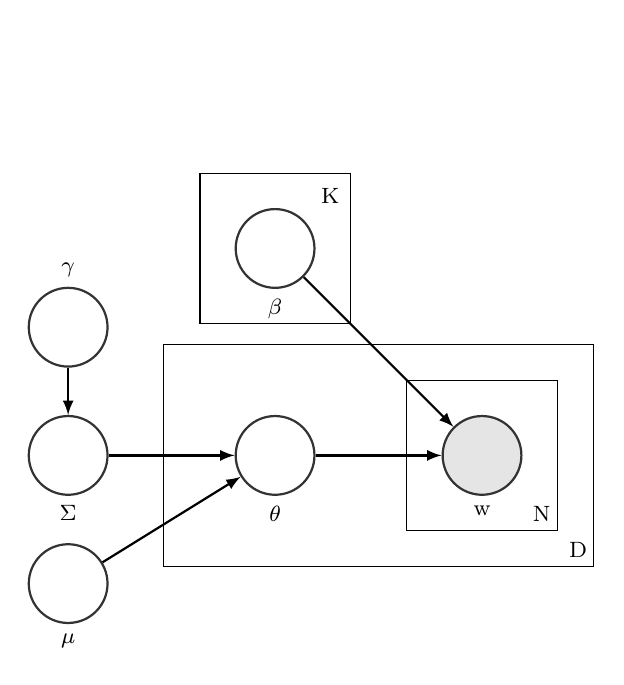
\begin{tikzpicture}
\tikzstyle{main}=[circle, minimum size = 10mm, thick, draw =black!80, node distance = 16mm]
\tikzstyle{connect}=[-latex, thick]
\tikzstyle{box}=[rectangle, draw=black!100]
  % sigma
  \node[main] (sigma) [label=below:$\Sigma$] { };    
  % mu
  \node[main] (mu) [yshift=1cm, below=of sigma, label=below:$\mu$] { };
  % gamma
  \node[main] (gamma) [yshift=-1cm, above=of sigma, label=above:$\gamma$] { };
  % eta
  \node[main] (theta) [right=of sigma,label=below:$\theta$] { };
  % z
%  \node[main] (z) [right=of theta,label=below:z] {};
  % beta
  \node[main] (beta) [above=of theta,label=below:$\beta$] { };
%  \node[main] (beta) [left=of psi,label=below:$\beta$] { };
  \node[main, fill = black!10] (w) [right=of theta,label=below:w] { };
  \path (gamma) edge [connect] (sigma)
  		(sigma) edge [connect] (theta)
  		(mu) edge [connect] (theta)
        (theta) edge [connect] (w)
%		(z) edge [connect] (w)
		(beta) edge [connect] (w);
%		(beta) edge [connect] (psi);
  \node[rectangle, inner sep=4.4mm,draw=black!100, fit= (beta)] {};
  \node[rectangle, inner sep=4.4mm, fit= (beta), label=below right:K, xshift=-5mm, yshift=18.5mm] {};
  \node[rectangle, inner sep=0mm, fit= (w),label=below right:N, , xshift=0mm] {};
  \node[rectangle, inner sep=4.4mm,draw=black!100, fit=  (w)] {};
  \node[rectangle, inner sep=4.6mm, fit= (w),label=below right:D, xshift=0mm] {};
  \node[rectangle, inner sep=9mm, draw=black!100, fit = (theta) (w)] {};
\end{tikzpicture}
\caption{Graphical model for TECTM}
\label{graph:lkjtm}
\end{figure}
% Generative process
The generative process of the $ d^{th} $ document is the following:\\
\begin{algorithm}[H]
Initialize hyperparameters $ \gamma $, $ \mu $\\
Sample Cholesky factor $ L\sim \text{LKJChol}(\gamma)$\\
\For{document d in D}{
Sample topic distribution $ \theta_d\sim \mathcal{LN}(\mu,LL^\top) $\\
\For{word position n in $ N_d $}{
Sample word $ w_{d,n}\sim \text{Cat}(\theta_d^\top\sigma(\rho^\top\alpha)) $
}
}
\caption{Generative Process for TECTM}
\label{algorithm:lkjtm}
\end{algorithm}
From algorithm \ref{algorithm:lkjtm}, starting from step 1, the topic proportion $ \theta_d $ is drawn from the logistic-normal distribution $ \mathcal{LN}(\cdot) $ with zero mean and identical covariance.
From Step 2-a, for each word position $ n $ in document $ d $, a topic assignment to word $ w_{dn} $ is drawn from categorical distribution $ Cat(\theta_d) $ parameterized by topic proportion $ \theta_d $
Step 2-b, the model draw a word from embedding of the vocabulary $ \rho $ and the assigned topic embedding $ \alpha_{z_{dn}} $ to draw the observed word from the assigned topic, as given by $ z_{dn} $. The embedding is applied softmax function to make them topic distribution.
The TECTM likelihood uses a matrix of word embedding $ \rho $, a representation of the vocabulary in a lower dimensional space. In practice, it can either rely on previously fitted embeddings as part of the fitting procedure, it simultaneously finds topics and an embedding space.
% TODO LKJ Correlation Distribution Formulation
\subsection{LKJ Correlation prior}
The LKJ Correlation prior LKJChol a A Cholesky factor of lower triangle matrix L, from a decomposed LKJ correlation distribution. The product of lower triangular matrix $ LL^\top $ reconstruct the correlation matrix
\begin{align*}
\Sigma = LL^\top
\end{align*}
A covariance matrix can be reconstructed in following fashion.
In our implementation, we don't scale the covariance matrix with variance $ \sigma $, which is simply a correlation matrix.
% TODO Transformer Embeddings
\subsection{Transformer Embeddings}
Following the ETM architecture, we modify topic-word distribution as an embedding and put transformer embedding to work into it. 
\begin{equation}\label{eq:ch4_transformer_embedding}
\beta\sim\text{softmax}(\rho^\top\alpha)
\end{equation}
Equation \ref{eq:ch4_transformer_embedding}, the topic-word distribution is composed of the dot product of transformer embedding $ \rho\in\mathbb{R}^{L\times V} $ representing the word vector in L-dimension of continuous space and topic matrix $ \alpha\in\mathbb{R}^{L\times K} $ mapping the L dimension vector into K-dimension of topic proportions.
% Marginal Likelihood
\subsection{Marginal Likelihood}
To compute the parameters of the model, we first compute the log-marginal likelihood. In equation \ref{eq:ch4_marginal_likelihood}, the marginal likelihood is parameterized by transformer embedding $ \rho $ and topic embedding $ \alpha $, which is for constructing topic-word proportion $ \beta $ as referenced in equation \ref{eq:ch4_transformer_embedding},
\begin{equation}\label{eq:ch4_marginal_likelihood}
\mathcal{L}(\rho,\alpha)=\sum_{d=1}^{D}\log p(w_d|\rho,\alpha)
\end{equation}
the marginal probability for $ p(w|\alpha) $ on $ d $-th document,
\begin{align}
p(w_d|\rho,\alpha)=\int p(\theta_d|\mu,\Sigma)\prod_{n=1}^{N_d}p(w_{dn}|\theta_d,\rho,\alpha)d\theta_d
\end{align}
the conditional distribution $ p(w_{dn}|\theta_d,\alpha) $ marginalize out the topic assignment $ z_{dn} $ by collapsing parameters transformation $ w\sim \theta^\top\beta $,
\begin{align}
p(w_{dn}|\theta_d,\rho,\alpha)=\text{Cat}\left(\sum_{k=1}^{K}\sigma(\theta_{dk}\beta_{k})\right)
\end{align}
as always, computing integral for posterior is intractable, approximate inference is necessary to estimate the true parameter from the integral.
%where $ \beta $ represent the topic-word distribution, composed of transformer embedding $ \rho $ and topic embedding $ \alpha $, in such case, the vocab $ v $ represent the proportion of topic $ k $ that $ \beta_{kv} $ becomes,
%\begin{align}
%\beta_{kv}=\text{softmax}(\rho_v^\top\alpha_k).
%\end{align}
% TODO move this part (amortized inference)
%then we take the amortized inference to take out neural network for the representation,
%\begin{align}
%p(w_{d}|N(\mu_\theta(w),\sigma_\theta(w)),\beta)=\mathbb{E}_{\theta\sim N(\mu_\theta(w),\sigma_\theta(w))}\left[w_d^\top\sigma(\beta\theta)\right]
%\end{align}
%then apply reparametrization trick $ \theta=\mu+\sigma^{1/2}\epsilon $ to reduce the construction for in following term\\
%\begin{align}
%p(w_{d}|\mu_\theta(w)+\epsilon\sigma^{1/2}_\theta(w),\beta)=\mathbb{E}_{\epsilon\sim N(0,1)}\left[w_d^\top\sigma(\beta(\mu_\theta(w)+\epsilon\sigma^{1/2}_\theta(w)))\right]
%\end{align}
%% Joint Distribution
\subsection{Joint Distribution}
We give a description of the joint distribution, $ W,Z,\theta $ and $ \Sigma $ are variables and $ \beta, \mu $ and $ \gamma $ are latent variables. $ W $ is the word likelihood from the document collections, $ Z $ represents the topic-word assignment, $ \theta $ models the topic distribution for each document, and $ \Sigma $ is the covariance matrix which depends on the document-topic distribution $ \theta $.
\begin{align*}
p(W,Z,\theta,\Sigma|\beta,\mu,\gamma)&=p(W|Z)p(Z|\theta)p(\theta|\mu,\Sigma)\\
&=p(\Sigma|\gamma)\prod_{d=1}^{D}p(\theta_d|\mu,\Sigma)\prod_{n=1}^{V}p(z_{d,n}|\theta_d)p(w_{d,n}|z_{d,n},\beta)
\end{align*}
by taking  log on the joint probability, we obtain a objective function for optimization
\begin{align*}
\log p(W,Z,\theta,\Sigma|\beta,\mu,\gamma)=&\sum_{d=1}^{D}\left[\log p(\theta_d|\mu,\Sigma)+\sum_{n=1}^{V}\left[\log p(z_{d,n}|\theta_d)+\log p(w_{d,n}|z_{d,n},\beta)\right]\right]\\
&+\log p(\Sigma)
\end{align*}
\section{Inference and Estimation}
% Inference Equation
% Variational Inference
% KL-divergence for the logistic normal distribution
\subsection{Evidence Lower Bound(ELBO)}\label{ch4:2} To perform Variational inference, it is essential to derive the Evidence Lower Bound (ELBO) first as the objective function for the optimization. By 
\begin{align}\label{eq:elbo_1}
\mathcal{L}\geq&\mathbb{E}_q[\log p(W,Z,\theta,\Sigma)]-\mathbb{E}_q[\log q(Z,\theta,\Sigma)]\\
=&\sum_{d=1}^{D}\sum_{n=1}^{V}\mathbb{E}_q[\log p(w_{d,n}|z_{d,n},\beta)]+\sum_{d=1}^{D}\sum_{n=1}^{V}\mathbb{E}_q[\log p(z_{d,n}|\theta_d)]\\
&+\sum_{d=1}^{D}\mathbb{E}[\log p(\theta_d|\mu,\Sigma)]+\mathbb{E}_q[\log p(\Sigma|\gamma)]-\sum_{d=1}^{D}\sum_{n=1}^{V}\mathbb{E}_q[\log q(z_{d,n}|\alpha_{d,n})]\\
&-\sum_{d=1}^{D}\mathbb{E}_q[\log q(\theta_d|\lambda_d,\nu_d)]-\mathbb{E}_q[\log q(\Sigma|\phi)]
\end{align}
% TODO Monte Carlo Estimate
The expectation log likelihood term in \ref{eq:elbo_1} can be efficiently appriximated by the Monte Carlo sampling method,
\begin{align}\label{eq:elbo_2}
\mathcal{L}\approx\frac{1}{S}\sum_{s=1}^{S}p(W|\theta^{(s)})
\end{align}
\paragraph{Collapsing Parameters}
\begin{align}\label{eq:elbo_3}
\mathcal{L}&\geq\sum_{d=1}^{D}\int\int q(\theta_d)\log\frac{p(W_d|\theta_d,\beta)p(\theta_d|\mu,\Sigma)p(\Sigma|\gamma)}{q(\theta_d)q(\Sigma)}d\theta_d d\Sigma\\
&=\sum_{d=1}^{D}\left(\mathbb{E}_{q(\theta_d)}\left[\log p(W_d|\theta_d,\beta)\right]-KL(q(\theta_d)||p(\theta_d|\mu,\Sigma))\right)-KL(q(\Sigma)||p(\Sigma|\gamma))
\end{align}
Here we define amortized inference, a optimization technique which perform inference by defined neural networks. $ \mu_\theta(w) $ and $ \sigma_\theta(w) $ are two inference networks take input from the word $ w $. Then a output is generated by the Normal distribution parameterized by $ \mu_\theta(w) $ and $ \sigma_\theta(w) $.
\begin{align}\label{eq:elbo_4}
=&\sum_{d=1}^{D}\left(\mathbb{E}_{q(\theta_d)}\left[\log p(w_d|\mathcal{LN}(\mu_{\theta_d}(w_d),\sigma_{\theta_d}(w_d)),\beta)\right]-KL(q(\theta_d)||p(\theta_d|\mu,\Sigma))\right)\\
&-KL(q(\Sigma)||p(\Sigma|\gamma))
\end{align}
To apply reparameterization trick, we take transformation from normal distribution to $ \theta=\mu+\epsilon\sigma^{1/2} $ where $ \epsilon\sim N(0,1) $, as  equation \ref{eq:elbo_5}
\begin{align}\label{eq:elbo_5}
=&\sum_{d=1}^{D}\left(\mathbb{E}_{q(\epsilon)}\left[\log p(w_d|\sigma(\mu_{\theta_d}(w_d)+\epsilon\sigma_{\theta_d}(w_d)),\beta)\right]-KL(q(\theta_d)||p(\theta_d|\mu,\Sigma))\right)\\
&-KL(q(\Sigma)||p(\Sigma|\gamma))
\end{align}
we also apply the minibatch to make able the model perform by subsampling the document collection. By equation \ref{eq:elbo_6}
\begin{align}\label{eq:elbo_6}
\tilde{\mathcal{L}}=&\frac{\mathcal{D}}{|\mathcal{B}|}\sum_{d\in\mathcal{D_B}}\left(\mathbb{E}_{q(\epsilon)}\left[\log p(w_d|\sigma(\mu_{\theta_d}(w_d)+\epsilon\sigma_{\theta_d}(w_d)),\beta)\right]-KL(q(\theta_d)||p(\theta_d|\mu,\Sigma))\right)\\
&-KL(q(\Sigma)||p(\Sigma|\gamma))
\end{align}
The KL-divergence for the logistic-normal distribution is given as equation \ref{eq:elbo_7} closed-form expression,
\begin{align}\label{eq:elbo_7}
\text{KL}(q(\theta_d)||p(\theta_d|\mu,\Sigma))=-\frac{1}{2}\left(tr(\sigma_1^{-1}\sigma_0)+(\mu_1-\mu_0)\Sigma_1^{-1}(\mu_1-\mu_0)-K+\log\frac{|\sigma_1|}{|\sigma_0|}\right)
\end{align}
so the ELBO then becomes \ref{eq:elbo_8}
\begin{align}\label{eq:elbo_8}
\tilde{\mathcal{L}}=&\sum_{d=1}^{D}\left[-\frac{1}{2}\left(tr(\sigma_1^{-1}\sigma_0)+(\mu_1-\mu_0)\Sigma_1^{-1}(\mu_1-\mu_0)-K+\log\frac{|\sigma_1|}{|\sigma_0|}\right)\right]\\
&+\mathbb{E}_{\epsilon\sim\mathcal{N}(0,I)}\left[w_d^\top\log\sigma(\beta(\mu_0+\sigma_0^{1/2}\epsilon))\right]-KL(q(\Sigma)||p(\Sigma|\gamma))
\end{align}
% TODO algorithm for the optimization here
\subsection{Optimization step}\label{ch4:3}
In algorithm \ref{algorithm:lkjtm_obj}, first initialize the model and variational parameters. Then, for each epochs, we obtain the transformer embedding $ \rho $ from transformer. After that, the topic embedding $ \beta $ is computed by taking softmax of dot-product of $ \rho $ and $ \alpha $. Then a minibatch $ \mathcal{B} $ is selected from the document for optimization. The number of minibatch is the document collection divides minibatch size where $ \#\text{minibatch}=\frac{\mathcal{D}}{|\mathcal{B}|} $. For each minibatch, the model takes a document and sample lower Cholesky matrix from LKJ Cholesky distribution(description see section \ref{ch2:lkj}). A topic assignment for document d $ \theta_d $ is sampled from logistic-normal distribution $ \mathcal{LN}(\mu,\sigma LL^\top\sigma) $, where $ \mu $ is sampled from half-Cauchy distribution and covariance is a transformation from equation \ref{eq:lkj_trans}. For each word position n, a word is sampled from the softmax of dot-product of transformer embedding $ \rho $ and NN weight $ \alpha $. After the sampling process for the document collection, we estimate the ELBO loss $ L_{ELBO} $ for the topic model, and the cross entropy loss $ L_{CrossEntropy} $. Remind that the topic model and transformer take input differently. The topic model part takes bag-of-words input, a document-vocabulary matrix $ D\times V $ counting the occurrence of vocabulary v in document d. While transformer take sequence of document as input. 
To calculate the loss of the model , we sum up the ELBO loss $ L_{ELBO} $ and cross entropy loss for transformer $ L_{CrossEntropy} $. Then a stochastic gradient is computed by backpropagation. a gradient step to . The process iterates until the maximum iteration is reached. 
\\
\begin{algorithm}[H]
Initialize model and variational parameters\\
\For{epoch $i=1,2,\dots N$}{
Compute the trnasformer embedding $ \rho $\\
Compute $ \beta=\text{softmax}(\rho^\top\alpha) $\\
Choose a minibatch $ \mathcal{B} $ of documents\\
\ForEach{document d in $ \mathcal{B} $}{
Compute $ \mu_d=\text{NN}(x_d;\nu_\mu) $\\
Compute $ \sigma_d=\text{NN}(x_d;\mu_\sigma) $\\
Sample $ L\sim \text{LKJChol}(\gamma) $ \\
Sample $\theta_d\sim\mathcal{LN}(\mu,\sigma LL^\top\sigma)$\\
\ForEach{word position n in docuemnt $ N_d $}{
Sample word $ w_{dn}\sim \text{softmax}(\beta_{w_{dn}}\theta_{d}) $
}
}
Estimate ELBO loss $ \text{L}_\text{ELBO}$ from Eq. \ref{eq:elbo_8}\\
Compute Transformer loss $ \text{L}_\text{CrossEntropy}$ from Eq. \ref{eq:crossentropy}\\
Compute the total loss $ \text{L}=\text{L}_\text{ELBO}+\text{L}_\text{CrossEntropy} $\\
Compute the stochastic gradient via backpropagation\\
Take a stochastic gradient step\\
Update model parameters ($\rho,\alpha,$)\\
Update variational parameters ($ \ $)
}
\label{algorithm:lkjtm_obj}
\caption{Topic modeling with the LKJTM}
\end{algorithm}
%\begin{algorithm}[H]
%Initial $ \theta^{(0)} $ randomly\\
%\While{Not Converge}{
%Sample a document d uniformly from dataset $ \mathcal{D} $\\
%For all k, initial $ \gamma^{d}_{k}=1 $\\
%\While{Not Converge}{
%\For{$ i=1,\cdots,N_d $}{
%\begin{align*}
%\phi_{ik}^{d}\propto\exp{\mathbb{E}}[\log\pi^d_k]+\mathbb{E}[\log\beta_{k,w_i^d}]
%\end{align*}
%}
%Set $ \gamma^{d}=\alpha+\sum_{i=1}^{N_d}\phi_i^d $
%}
%Take a stochastic gradient step $ \theta^{t}=\theta^{t-1}+\epsilon_t+\triangledown_\theta\mathcal{L}_d $
%}
%\caption{SVI for LDA}
%\end{algorithm}
\section{Results \& Evaluations}
In this chapter, we perform evaluation on our model and the other algorithms, the repository of our model is provided in github \footnote{\url{https://github.com/cwleung/LKJTM}}.
\subsection{Experiment Testing}
The experiment will be conducted with a number of existing proposed topic models as mentioned related work section above. We conduct the experiment with those baseline algorithms and evaluate them in terms of accuracy and running time. Some of the source code of competitive were provided by their authors in Github\footnote{For instance, Correlated Topic Model(CTM), \href{https://github.com/blei-lab/ctm-c}{https://github.com/blei-lab/ctm-c}}. The outcome result will be extensively studied and conclude the insight behind the algorithms and methodologies. Detail to be stated in section \ref{AD}. Our probabilistic part of model implemented using Pyro\cite{bingham_pyro_2019}, while the model optimization and transformer implementations are based on PyTorch\cite{paszke_automatic_2017}.
\subsection{Dataset}To evaluate the performance of the model, we selected \textit{20Newsgroups} and \textit{Reuters-21578} data sets in our evaluation stage. 20Newsgroups consist of 18,846 news group documents \footnote{\url{http://qwone.com/~jason/20Newsgroups/}} and the Reuters-21578 includes 10,788 documents in total. Both of the dataset will be preprocessed to remove stop-words and stemming before the evaluation. Both data set were separated into training/testing set for training and evaluation process. 
% 20newsgroups
\textit{20Newsgroups} data set contains around 20,000 newsgroups documents, which divided into 20 different groups. In the preprocessing stage, we remove the document with only one word. We filter the stop-words, remove the word with special characters. The frequency of words are limited to between 2\%-70\%. After the preprocessing, the data set was split into 11314, 7532 documents with 5453 vocabularies. 
% reuter 21578
\textit{Reuter-21578} data set is a collection of documents from Reuters newswire in 1987. After performing the preprocessing, the processed data set consist of 7769, 3019 documents for train/test documents with 1623 vocabularies.
\subsection{Data Preprocessing}
We perform data preprocessing, tokenization, stopword removal, lemmatization, and set the 
\subsection{Models}
We compare the model performance with a numbers of rivals. We take Latent Dirichlet Allocation (LDA)\cite{blei_latent_2003} as the baseline model. Other models include Transformer\cite{vaswani_attention_nodate}\footnote{Not a topic model, but we think it is worth to make comparison still.},  ProdLDA\cite{srivastava_autoencoding_2017} and Embedded Topic Model(ETM)\cite{dieng_topic_2019}.
% LDA
LDA model with mean-field inference \footnote{Adopted from \textmd{scikit-learn} library}
% ProdLDA
ProdLDA, a topic model learning using amortized inference to approximate the document-topic proportion.
% ETM
ETM model, a topic model built on top of ProdLDA model, uses dot-product of word embedding and topic embedding to represent the topic-word distribution $ \beta $.
\subsection{Algorithmic Settings}
% optimization algorithm
To perform posterior inference, we employed Stochastic Variational Inference (SVI) \cite{hoffman_stochastic_2013} for the optimization problem. We set the minibatch size to 1024 documents.
% Other model
For LDA, we applied the model provided from sklearn package (version 0.24.0) \footnote{Sklearn website \url{https://scikit-learn.org/stable/index.html}}. For ETM, we run the experiment with the parameter suggested \cite{dieng_topic_2019}. For ProdLDA, we perform optimization with inference network architecture as described in the paper \cite{srivastava_autoencoding_2017}. 
% epochs
To train the models, every model run on 200 epochs to give the best performance. 
% learning rate
To perform optimization, we use Adam for the gradient ascent algorithm, and we set the learning rate to 2e-3.
% l2-regularization factor
we use $ l2 $-regularization to the 1e-5,
% inference network [size, activation function, dropout, batch-norm]
We applied the settings from \cite{srivastava_autoencoding_2017} to perform amortized inference. The inference architecture included 100 dimension of hidden layers. 
% embedding dimension 512
The dimension for embedding $ \rho $ are set to 128.
% Transformer settings
For the Transformer model settings, we define the sequence length to 20, number of head to 8, and 6 layer stacks of transformer encoder and 128 hidden dimension.
\subsection{Quantitative Result}
In this section, we evaluate the model with the following metric adopted from \cite{dieng_dynamic_2019}: Perplexity, Topic Coherence (TC), Topic Diversity (TD). %and Topic Quality (TQ).\begin{center}
\begin{table}[h]
\centering
\begin{tabular}{lllllll}
\hline
\#Topic     & \multicolumn{3}{c}{k=20} & \multicolumn{3}{c}{k=50} \\
Metrics     & PPL      & TC      & TD  & PPL      & TC      & TD  \\
\hline
LDA         & 2425.9   & 0.183   &  0.754   & \textbf{2521.7}   & 0.149   & 0.742    \\
ProdLDA     & 5652.0   & 0.107   &   0.906  & 5654.1   & 0.074   &     \\
ETM         & \textbf{2709.7}   & 0.153   &  0.486   & 2729.2   & 0.132   & 0.265    \\
Our model   & 3444.1   & \textbf{0.206}   &     & 3705.0   & \textbf{0.199}   &    \\
\hline
\end{tabular}
\captionof{table}{Result for 20Newsgroups dataset\label{tbl:result1}}
\end{table}
\begin{table}[h]
\centering
\begin{tabular}{lllllll}
\hline
\#Topic     & \multicolumn{3}{c}{k=20} & \multicolumn{3}{c}{k=50} \\
Metrics     & PPL     & TC     & TD    & PPL     & TC     & TD    \\ \hline
LDA         & 464.5   & 0.204  & 0.692 & \textbf{510.1}   & 0.155  &  0.580     \\
ProdLDA     & 1599.3  & -0.38  & \textbf{0.872} & 1568.3  & -0.411 & \textbf{0.686} \\
ETM         & \textbf{375.3}   & 0.207  & 0.382 & 629.9   & 0.127  & 0.113 \\
Our model   & 826.3   & \textbf{0.250}  & 0.69  & 805.5   & \textbf{0.253}  & 0.508 \\ \hline
\end{tabular}
\captionof{table}{Result for Reuters-21578 dataset\label{tbl:result2}}
\end{table}
\paragraph{20Newsgroups}On the result from table \ref{tbl:result1}, display that our model has outperform the other model by TC score. On perplexity score, ETM obtain the best score when $ k=20 $ and LDA when $ k=50 $. Since Transformer is not a topic model actually, it got a negative score on TC, which refers it cannot retrieve any useful topic from documents.
\paragraph{Reuters-21578}
% Reuter-21578
On the dataset Reuter-21578, the LDA perform the best in perplexity and ETM when $ k=50 $. And our model still perform the best on topic coherence on both number of topic. 
%
Apparently our model outcome a relatively high topic coherence score but a high perplexity. To investigate the problem, we analyze the metric performance per training epoch.

\subsection{Training}
From figure \ref{fig:loss_20ng_20t}, \ref{fig:loss_20ng_50t}, display the training process of the training loss and log probability by 200 epochs. From \ref{fig:eval_20ng_20t}, \ref{fig:eval_20ng_50t}, we observe that the TD score and TC score increase monotonically, however, the perplexity increases throughout the epochs. 
\subsection{Qualitative Result}The proposed model will be evaluated with a number of specifically selected topic and examined with their performance separately. The result will be exhaustively compared with other existing models.\\
From table \ref{tbl:t3}, we have selected some topic words each model generated from 20Newsgroups when $ k=20 $. The topics represent space, operating system, religion, encryption and guns respectively. Our model has shown capability on capturing key words from each topic, such as on topic "space": \textit{nasa}, \textit{space}, \textit{jpl}, \textit{moon}, \textit{earth}, \textit{station}, \textit{flight} are the outputs.
\begin{table}[ht]
\centering
%\scriptsize
\begin{tabular}{llll}
\hline
Our Model  \\ \hline
\textbf{nasa }gov \textbf{space jpl moon earth station flight }research digex\\
\textbf{windows window }problem \textbf{dos }running \textbf{file mouse }mit de ms\\
\textbf{god jesus christian }people faith bible time church good things\\
\textbf{key }chip \textbf{encryption }clipper \textbf{security }\textbf{privacy }government \textbf{keys }public escrow\\
\textbf{gun }people control government \textbf{guns weapons }american make clinton state \\ \hline
\hline
ProdLDA  \\ \hline
\textbf{nasa} \textbf{space} gov people \textbf{station} \textbf{time} \textbf{orbit} dc program shuttle \\
\textbf{scsi} \textbf{drive} \textbf{controller} max \textbf{drives} \textbf{ide} senior \textbf{tape} time people \\
\textbf{god jesus atheists christian bible religion atheism christians} word truth \\
\textbf{key crypto} session nt chips chip \textbf{serial} dos \textbf{keys} \textbf{encrypted} \\
\textbf{gun }people god religion writes life morality ohio argument question \\ \hline
\hline
LDA  \\ \hline
\textbf{space, nasa}, gov, access, \textbf{launch, earth}, digex, \textbf{moon, orbit}\\
\textbf{file, window, program, ftp}, \textbf{files}, \textbf{server}, \textbf{image, graphics, windows}\\
\textbf{god}, people, \textbf{jesus}, \textbf{christian}, \textbf{bible}, writes, life, \textbf{christians}, time\\
\textbf{key}, \textbf{encryption}, chip, clipper, \textbf{keys}, \textbf{security}, \textbf{government}, \textbf{privacy}\\
\textbf{gun, guns, law, police}, people, \textbf{weapons, crime, fbi}, control
\\ \hline
\hline
ETM  \\ \hline
\textbf{space, nasa}, gov, mr, president, health, research, year, center\\
\textbf{windows, file, window, program, files, server}, \textbf{version}, dos, \textbf{image}\\
\textbf{god}, people, \textbf{jesus}, \textbf{christian}, \textbf{israel}, \textbf{bible}, \textbf{jews}, \textbf{christians}, \textbf{israeli}\\
\textbf{key, encryption}, chip, clipper, \textbf{keys}, \textbf{privacy}, \textbf{security}, technology, government\\
\textbf{gun}, people, government, \textbf{law}, state, \textbf{guns}, article, \textbf{weapons}, control
\\ \hline
\end{tabular}
\captionof{table}{Top-9 words for each topic from 5 topics selected\label{tbl:t3}}
\end{table}
\begin{figure}[h]
\centering
\subcaptionbox{Log probability}{\includegraphics[width=0.50\textwidth]{figures/0908/log_prob_20t}}%
\hfill
\subcaptionbox{Negative ELBO}{\includegraphics[width=0.50\textwidth]{figures/0908/elbo_20t}}%
\hfill
\caption{20Newsgroups (k=20)}
\label{fig:loss_20ng_20t}
\end{figure}
\begin{figure}
\centering
\subcaptionbox{Log probability}{\includegraphics[width=0.50\textwidth]{figures/0908/log_prob_50t}}%
\hfill
\subcaptionbox{Negative ELBO}{\includegraphics[width=0.50\textwidth]{figures/0908/elbo_50t}}%
\hfill
\caption{20Newsgroups (k=50)}
\label{fig:loss_20ng_50t}
\end{figure}
\begin{figure}
\centering
\subcaptionbox{Topic Diversity}{\includegraphics[width=0.50\textwidth]{figures/0908/td_20t}}%
\hfill
\subcaptionbox{Topic Coherence}{\includegraphics[width=0.50\textwidth]{figures/0908/tc_20t}}%
\hfill
\subcaptionbox{Perplexity}{\includegraphics[width=0.50\textwidth]{figures/0908/ppl_20t}}%
\hfill
\caption{20Newsgroups (k=20)}
\label{fig:eval_20ng_20t}
\end{figure}
\begin{figure}
\centering
\subcaptionbox{Topic Diversity}{\includegraphics[width=0.50\textwidth]{figures/0908/td_50t}}%
\hfill
\subcaptionbox{Topic Coherence}{\includegraphics[width=0.50\textwidth]{figures/0908/tc_50t}}%
\hfill
\subcaptionbox{Perplexity}{\includegraphics[width=0.50\textwidth]{figures/0908/ppl_50t}}%
\hfill
\caption{20Newsgroups (k=50)}
\label{fig:eval_20ng_50t}
\end{figure}
\subsection{Visualization}
To clearly demonstrate the representation for , we applied t-SNE to map the topic-word representation into 2-dimension continuous space. In figure \ref{fig:tsne20t25w2} and \ref{fig:tsne50t25w0}, demonstrate the t-SNE visualization of the topic-word distribution for 20Newsgroups for k=20 and k=50.
\begin{figure}
\centering
\includegraphics[width=1\linewidth]{figures/0908/tsne_20t_25w_2}
\caption{Visualization \#Topics:20}
\label{fig:tsne20t25w2}
\end{figure}
\begin{figure}
\centering
\includegraphics[width=1\linewidth]{figures/0908/tsne_50t_25w_0}
\caption{Visualization \#Topics:50}
\label{fig:tsne50t25w0}
\end{figure}
\subsection{Discussion}
The result exhibits our model has a outstanding performance on obtaining high quality topic words over various of predefined topic numbers. In two of the metric we compared, topic coherence and topic diversity, 
%\chapter{Correlated Topic Model with Transformer Embeddings}\label{ch5}
%In most of the real-life cases, the context (or formally topic information), that to be mentioned in the media such as news and documents are changing over time. Also, the word meaning and slang at the time may not valid on other span of time.
In this chapter, we expand the embedded topic model to deal with times-series task, namely Dynamic Transformer embedded topic model. The model utilizes the time information 
\section{Model description}
\paragraph{}The TETM utilizes the Transformer as embedding to the topic-word representations. To compare with the original topic model, the word-topic distribution $ \beta $ is the 
First, the topic embedding embeds the vocabulary into L-dimensional space, which is by Transformer embedding. Second, the context embedding maps the embedding into K-dimensional space . 
In the generative process, the LKJTM uses the topic embedding to form a per-topic vector to represent the meaning over the vocabulary. 
% Graphical model for the DTM
% Embedding
\paragraph{}
To express the way word embedding to be applied in our model, $ \rho\in\mathbb{R}^{V\times L} $ is the Transformer embedding in the model. $ \rho_v $ is a vector represents the embedding of vocabulary on n-th index.
% Time variables
To explain the way our model capture time-related information from document set, we here discuss variables change over time. The topic embedding $ \{\alpha^{(t)}_k\}^{T}_{t=1}\in\mathbb{R}^{L} $ is a vector distributed at specific k topic.
% theta, eta
Topic proportion $ \theta_d $ is same as typical topic model, which a simply a vector represent proportion for each topic on document d.
The latent variable $ \eta $ decide the topic proportion holds on each timestamp ranged between $ 1, \dots, T $. 
% word vector training process $\tilde{w}$
\subsection{Time-dependent variables}
% alpha
The topic-word proportion is contributed 
$ p(\alpha^{t}|\alpha^{t-1})=\mathcal{N}(\alpha_{t-1},\gamma^2I) $\\
% eta, theta
The generation for document-topic proportion is a state-space Markov model. The $ \eta_{1:T}\in\mathbb{R}^{K} $ is a Gaussian process latent variable model that contributes the topic proportion mean for variable $ \theta $. $ \eta_t\sim\mathcal{GPLVM}(0,\mathcal{K}_{\theta}) $ 
% zero mean, rbf kernel
$ \theta_t|\eta_t\sim\mathcal{LN}(\eta_{t-1},\xi^2I) $ 
\subsection{Amortized variational distribution}
% Generative process
The generative process is as following:\\
\begin{algorithm}[H]
Initialize hyperparameters\\
Draw topic embedding $ \alpha_{1:K}^{(1:T)}\sim\mathcal{N}(\alpha_k^{(t-1)},\gamma^2I) $\\
Draw topic proportion mean $ \eta_{1:T}\sim\mathcal{GP}-\mathcal{LVM}(0,\mathcal{K_\theta}) $\\
\For{document d in D}{
Sample topc proportion $ \theta_{t_d}\sim\mathcal{LN}(\eta_{t_d},\xi^2I) $\\
%Sample topic distribution $ \theta_d\sim \mathcal{LN}(\mu,\sigma LL^\top\sigma) $\\
\For{word position n in $ N_d $}{
Sample word $ w_{d,n}\sim\text{Cat}(\theta\sigma(\rho^\top\alpha^{(t_d)})_{z_{d_n}}) $
%Sample word $ w_{d,n}\sim \sigma(\theta_d(\rho^\top\alpha)_{\cdot,w_{d,n}}) $
}
}
\caption{Generative Process for DTM}
\label{algorithm:ldtm}
\end{algorithm}
From algorithm \ref{algorithm:ldtm}, first the model draws a topic embedding $ \alpha_{1:K}^{1:T} $ from normal distribution at time $ 1,\dots,T $. At time step 0, the topic embedding initialized at $ \mathcal{N}(0,I) $.
% topic proportion
Then a topic mean $ \eta_t\in\mathbb{R}^{K} $ over timestamps is generated from the Gaussian Process latent variable model(GPLVM), which performs inference a dimensions of topic K from number of vocabularies V dimension. Specifically, taking bag-of-word by time $ w_t $, which is collected by categorizing the document by time and group them into word count matrix by timestamp. And then a normalization is performed to make sure the words in different timestamp are in same proportion.
% sample topic proportion
For each document, draw a topic proportion $ \theta_{d} $ from logistic-normal distribution $ \mathcal{LN}(\cdot,\cdot) $ condition on topic mean $ \eta_{t_d} $ at the timestamp t of document d, and the variance $ \xi^2I $.
% for word
After that, for each word position n in $ N_d $, a word is drawn from the dot-product of word embedding $ \rho $ and topic embedding $ \alpha^{(t_d)}_{d} $ at timestamp $ t_d $. 
\subsection{Joint Distribution}
To describe the joint distribution for the model, equation \ref{eq:dtetm_joint}
\begin{align}\label{eq:dtetm_joint}
p(w,\theta,\eta,\alpha)=\prod_{d=1}^{D}\prod_{n=1}^{N_d}p(w_{d,n}|\theta_d,\alpha^{(t_d)})\prod_{d=1}^{D}p(\theta_d|\eta_{t_d},w_d)\prod_{t=1}^{T}p(\eta_t|w_t)\prod_{k=1}^{K}\prod_{t=1}^{T}p(\alpha_k^{(t)})
\end{align}
For the bag-of-word input, we have V vocabularies over D documents. A number of K topics are defined to be introduced in the model. Each document is labeled a timestamp t over a time span between $ 1,\dots,T $.
\begin{enumerate}
\item $\theta_d\in\mathbb{R}^{D\times K}$ is the topic proportion for document d.
\item $\eta_{t_d}\in\mathbb{R}$ is the topic proportion at time t of document d.	
\item $ w_d \in\mathbb{R}^{V}$ is the bag-of-word of distribution at document d.
\item $ w_t \in\mathbb{R}^{V}$ is the bag-of-word of distribution at time t, which we arranged the documents in different timestamp and group them into bag-of-word representation in dimension $ \mathbb{R}^{V\times T} $
\item $\alpha_k^{(t)}\in\mathbb{R}^{V}$ is the topic embedding for topic k at time t. The topic embedding demonstrates the vocabulary representations on the specific time stamp for the document.
\item $ \rho\in\mathbb{R}^{W\times L} $ is the transformer embedding that maps the words into L dimension of continuous latent space. 
\end{enumerate}
\begin{enumerate}
\item $ p(w_{d,n}|\theta_d,\alpha^{(t_d)}) $
\item $ p(\theta_d|\eta_{t_d},w_d) $
\item $ p(\eta_t|w_t) $
\item $ p(\alpha_k^{(t)}) $
\end{enumerate}
%\section{Inference and Estimation}
Since the posterior is intractable to compute, we apply variational inference to approximate the parameters for the log-marginal likelihood.
\subsection{Variational Distribution}
To begin with, we first setup variational distribution to approximate the parameter of the model. 
\begin{equation}
q(\theta,\eta,\Sigma,\alpha)=\prod_{d=1}^{D}q(\theta_d|w_d,\eta_{t_d},\Sigma_{t_d})\prod_{t=1}^{T}q(\eta_t|w_t)q(\Sigma_{t}|\gamma_{t})\prod_{k=1}^{K}q(\alpha_k^{(t)})
\end{equation}
The variational distribution for topic proportion $ q(\theta_d|\eta_{t_d},w_d) $ is logistic-normal distribution. We applied amortized inference to approximate the model, which the mean and covariance matrix is generated by two inference network $ \mu_\phi $ and $ \sigma_\phi $ taking bag-of-word input $ w_d $ at each document d and residual input $ \eta_{t_d} $ end up $ \mathbb{R}^{D\times (V+K)} $ dimension in the input space.
% residual input part
The output for time-topic proportion is applied to the residual connection on the amortized inference of document-topic proportion $ \theta $. The inference network for variational parameter $ \phi $ take the residual input from stacked input: both $ \mathbb{R}^{V} $ bag-of-words vectors $ w_d $, and the $ \mathbb{R}^{K} $ time-topic proportion $ \eta_{t_d} $.
Then we transform the  using reparameterization trick.
% layernorm
To perform amortized inference for $ \theta $, we apply Layer Normalization\cite{ba_layer_2016} to normalize the input vectors. The LayerNorm performs normalization over features, which enables a better training. Also, it is more stable than batch normalization for training while the batch size is pretty small. And thus it is able to maintain a lower variance than batch normalization does throughout the training loop.
\begin{align}\label{eq:ch5_variational_theta}
q(\theta_d|\eta_{t_d},w_d,\Sigma_{t_d})&=\mathcal{N}(\mu_\phi(x),\Sigma_{t_d})\\
x&=\text{LayerNorm}([w_d,\eta_{t_d}])
\end{align}
% TODO eta variational distribution, how to write the decoder encoder format
The variational distribution for $ q(\eta_t|w_t) $ is basically the normal distribution parametrized by two inference network, which takes the input from bag-of-word $ w_d $ and the variable from \cite{lawrence_learning_2007}, L is the dimension for latent input space, V is the token size.
\begin{align}\label{ch5:eq_var_eta}
q(\eta_t|w_t)=\int\prod_{i=1}^{V}q(w_i)\prod_{d=1}^{L}p(f_d|u_d,W)q(u_d)du_d
\end{align}
% alpha
The variational distribution for $ q(\alpha_k^{(t)}) $ is the embedding is parameterized mean $ \mu_{\varphi} $ and $ \sigma_{\varphi} $ conditioned on local parameter $ \varphi $. Notice that $ \varphi $ is not a variational parameter as usual amortized inference.
\begin{align}\label{ch5:eq_var_alpha}
q(\alpha^{(t)})=\mathcal{N}(\mu_\varphi^{(t)},\sigma_\varphi^{(t)})
\end{align}
% reparameterization trick
both variational distribution $ q(\theta_d|\eta_{t_d}, w_d) $ and $ q(a^{(t)}) $ applied reparameterization trick \cite{kingma_auto-encoding_2014} with transformation $ \mathcal{N}(\mu,\sigma)\approx\mu+\epsilon\sigma^{1/2}, \epsilon\sim \mathcal{N}(0,1) $, to avoid high variance on the variational variables.
% Inference Equation
\subsection{Evidence lower bound (ELBO)}
We take the log marginal likelihood from eq. \ref{eq:dtetm_joint}. Noted the given equation could derive the ELBO by simply applying the Jensen inequality. For sake of simplicity, we decompose the marginal likelihood two parts, the document-topic proportion part and the time-topic proportion part. Then summing up the terms as eq. \ref{ch5:eq_elbo1}. In such way, we are able to derive a ELBO without calculating the KL-divergence for $ q(\eta_{t_d}) $ and $ p(\eta_{t_d}|w_t) $. And so we could obtain the ELBO for $ \log p(\eta_{t_d}|w_t) $ conveniently from \cite{titsias_bayesian_nodate}.
%\begin{align}\label{eq:ch6_elbo1}
%\log p(w_d|\theta_d,\alpha)=&\sum_{d=1}^{D}p(\alpha^{(t_d)}|\alpha^{(t_d-1)})\iint\log p(w_d|\theta_d,\eta_{t_d},\alpha^{(t_d)})p(\theta_d|\eta_{t_d},w_n,\Sigma_{t_d})p(\eta_{t_d}|w_t)d\theta_{d}d\eta_{t_d}\\
%=&\sum_{d=1}^{D}\int\log p(w_d|\theta_d,\eta_{t_d},\alpha^{(t_d)})p(\theta_d|\eta_{t_d},w_n,\Sigma_{t_d})\\
%+\log p(\eta_{t_d}|w_t)d\theta_dd\eta_{t_d}
%\end{align}
%define the ELBO
%\begin{align*}
%\mathcal{L}_1\geq\sum_{d=1}^{D}\iiint q(\theta_d)q(\eta_{t_d})q(\Sigma_{t_d})\frac{p(w_{d,n}|\theta_d,\rho,\alpha^{(t_d)})p(\theta_d|\eta_{t_d},w_d,\Sigma_{t_d})p(\Sigma_{t_d}|\gamma_{t_d})}{q(\theta_d)q(\eta_{t_d})q(\Sigma_{t_d})}d\theta_{d}d\eta_{t_d}d\Sigma_{t_d}
%\end{align*}
\begin{align}\label{ch5:eq_elbo1}
\mathcal{L}\geq&\mathbb{E}_q[\log p(W,\theta,\eta,\Sigma,\alpha|\rho,\gamma)]-\mathbb{E}_q[\log q(\theta,\eta,\Sigma,\alpha)]\notag\\
=&\sum_{d=1}^{D}\sum_{n=1}^{V}\mathbb{E}_q[\log p(w_{d,n}|\theta_d,\rho,\alpha^{(t_d)})]+\sum_{d=1}^{D}\mathbb{E}[\log p(\theta_d|\eta_{t_d},\Sigma_{t_d})]\notag\\
&+\sum_{t=1}^{T}\mathbb{E}_{q}[\log p(\eta_{t})]+\sum_{t=1}^{T}\mathbb{E}_q[\log p(\Sigma_{t})]+\sum_{t=1}^{T}\sum_{k=1}^{K}\mathbb{E}_{q}[\log p(\alpha_{k}^{(t)}|\alpha_{k}^{(t-1)})]\notag\\
&-\sum_{d=1}^{D}\mathbb{E}_q[\log q(\theta_d|\mu_{\phi}(x_d),\Sigma_{t})]-\sum_{t=1}^{T}\mathbb{E}_{q}[\log q(\eta_{t}|w_{t})]-\sum_{t=1}^{T}\mathbb{E}_q[\log q(\Sigma_{t}|\gamma_{t})]\notag\\
&-\sum_{t=1}^{T}\sum_{k=1}^{K}\mathbb{E}_q[\log q(\alpha_{k}^{(t)}|\alpha_{k}^{(t-1)})]
\end{align}
% second term
and by rearranging the terms, the ELBO can be represented as follows, where the first term is the reconstruction loss, and the remaining is the KL-divergence between the prior and variational distribution for its variational parameters.
\begin{align}\label{eq:ch5_elbo1}
=&\sum_{d=1}^{D}\sum_{n=1}^{V}\mathbb{E}_q[\log p(w_{d,n}|\theta_d,\rho,\alpha^{(t_d)})]-\sum_{d=1}^{D}\text{KL}(q(\theta_d|w_d,\eta_{t_d},\Sigma_{t_d})||p(\theta_d|\eta_{t_d},\Sigma_{t_d}))\notag\\
&-\sum_{t=1}^{T}\text{KL}(q(\eta_{t}|w_{t})||p(\eta_{t}))-\text{KL}(q(\Sigma_{t}|\gamma_{t})||p(\Sigma_{t}))\notag\\
&-\sum_{k=1}^{K}\text{KL}\left(q(\alpha_{k}^{(t)}|\alpha_{k}^{(t-1)})||p(\alpha_{k}^{(t)}|\alpha_{k}^{(t-1)})\right)
\end{align}
% separate the terms
For sake of simplicity, we separate the ELBO into three parts. We first derive the ELBO for the document-topic model part, denoted as $ \mathcal{L}_{1} $, we can obtain $ p(w_d,\theta_d,\alpha|\eta_{t_d})=p(w_d|\theta_d,\alpha^{(t_d)})p(\theta_{d}|\eta_{t_d})p(\alpha)$ by factorization. 
\begin{align}\label{eq:ch5_elbo_p1}
\mathcal{L}_{1}=&\sum_{d=1}^{D}\sum_{n=1}^{V}\mathbb{E}_q[\log p(w_{d,n}|\theta_d,\rho,\alpha^{(t_d)})]-\sum_{d=1}^{D}\text{KL}(q(\theta_d|w_d,\eta_{t_d},\Sigma_{t_d})||p(\theta_d|w_d,\eta_{t_d},\Sigma_{t_d}))\notag\\
&-\sum_{t=1}^{T}\text{KL}(q(\Sigma^\phi_{t}|\gamma_{t})||p(\Sigma_{t}))
%\sum_{d=1}^{D}\int q(\theta_d)\log\frac{p(w_d|\theta_{d},\alpha)p(\theta_d|\eta_{t_d},w_d)}{q(\theta_d)q(\eta_{t_d})}d\theta_d\\
%=&\sum_{d=1}^{D}\mathbb{E}_{ q(\theta_d|\eta_{t_d},w_d)}[\log p(w_{d}|\theta_d,\alpha^{(t_d)})]-\text{KL}(q(\theta_d|\eta_{t_d},w_t)||p(\theta_d|\eta_{t_d}))\\
\end{align}
% TODO monte carlo estimation
% minibatch
To speed up computation, we apply mini-batching as previous chapter
\begin{align}
\tilde{\mathcal{L}}_{1}\approx&\frac{|\mathcal{D}|}{|\mathcal{B}|}\sum_{d\in\mathcal{D}_{\mathcal{B}}}\bigg[\sum_{n=1}^{V}\mathbb{E}_q[\log p(w_{d,n}|\theta_d,\rho,\alpha^{(t_d)})]-\text{KL}(q(\theta_d|w_d,\eta_{t_d},\Sigma_{t_d})||p(\theta_d|w_d,\eta_{t_d},\Sigma_{t_d}))\bigg]\\
&-\sum_{t=1}^{T}\text{KL}(q(\Sigma^\phi_{t}|\gamma_{t})||p(\Sigma_{t}))
\end{align}
% expectation
The first term is the expected likelihood term for reconstructing the word $ w_{dn} $ from the model, where $ p(w_{d,n}|\theta_d, \rho,\alpha^{(t_d)}) $ is the log likelihood probability parameterized by the variational parameters $ \theta_d, \alpha^{t_d} $ and transformer embedding $ \rho $, which $ \sigma(\cdot) $ is the softmax function. The topic-word proportion is a dot product of transformer embedding $ \rho $ and $ \alpha^{(t_d)} $
\begin{align}
\mathbb{E}_{q(\theta_d)q(\alpha)}[\log p(w_{d,n}|\theta_d,\rho,\alpha^{(t_d)})]=\mathbb{E}_{\theta_d\sim\mathcal{N}(\mu_{\phi}(x),\Sigma^{\phi}_{t_d})}[w_{d,n}\sigma(\theta^\top(\rho^\top\alpha^{(t_d)}))_{d,n}]
\end{align}
and then apply the reparameterization trick to maintain a low-variance gradient estimate to the likelihood term, the transformation $ \theta_d=\mu_{\phi}(x)+(\Sigma^{\phi}_{t_d})^{1/2}\epsilon $, where $ \epsilon\sim\mathcal{N}(0,I) $ is gaussian noise variance.
% expectation 2
\begin{equation}\label{eq:ch5_reconstruction}
=\mathbb{E}_{\epsilon\sim\mathcal{N}(0,I)}\left[w_{d,n}\sigma((\mu_{\phi}(x_d)+(\Sigma^{\phi}_{t_d})^{1/2}\epsilon)^\top(\rho^\top\alpha^{(t_d)}))_{d,n}\right]
\end{equation}
% theta
The second term is the KL-divergence between $ p(\theta_d) $ and $ q(\theta_d) $, the distributions are logistic-normal distributions so can be represented in closed-form. So we simply derive the KL-divergence by substitution,
%\begin{align}\label{eq:ch5_kl_theta}
%\text{KL}(q(\theta_d|\mu_\phi,\sigma_\phi)||p(\theta_d|\eta_{t_d},w_d))=\frac{1}{2}\left(\log\frac{1}{\sigma_\varphi^2}+\sigma_\phi^2+(\mu_\phi-\eta_{t_d})^2-1\right)
%\end{align}
% eta
the variable x is the parameter stacked with bag-of-word $ w_d $ and residual input $ \eta_{t_d} $ from \ref{eq:ch5_variational_theta}
\begin{align}\label{eq:ch5_kl_theta}
&\text{KL}(q(\theta_d|\mu_{\phi}(x),\Sigma^{\phi}_{t_d})||p(\theta_d|\eta_{t_d},\Sigma_{t_d}))\notag\\
=&\frac{1}{2}\left(\text{tr}(\Sigma_{t_d}^{-1}\Sigma_{t_d}^{\phi})+(\eta_{t_d}-\mu_{\phi}(x_d))^\top\Sigma_{t_d}^{-1}(\eta_{t_d}-\mu_{\phi}(x_d))+\log\frac{|\Sigma_{t_d}|}{|\Sigma^{\phi}_{t_d}|}-K\right)
\end{align}
For the second part, we derive the ELBO for GPLVM, which the detailed derivation for the ELBO has been discussed in the original paper \cite{titsias_bayesian_nodate} as equation \ref{eq:ch5_elbo_p2}. $ w=\{w_t\}^{T}_{t=1}\in\mathbb{R}^{T\times V} $ is the observed data, which bag-of-words with respect to the word count by that timestamps over the documents. $ \eta=\{\eta_t\}^{T}_{t=1}\in\mathbb{R}^{T\times K} $, the latent variable distributes the topic proportion over time. Known that the dimension reduction is performed, as $ K<<V $, where the defined number of topic is supposed to be much smaller than the size of vocabularies.
% f_d, u_d, Z
$ f_d $ is the latent function which takes $ M $ inducing point $ u_d $, where M is the number of inducing points defined for the training process. And where $ u_d $ is conditioned at input locations $ Z\in\mathbb{R}^{M\times K} $. 
% phi, lambda
$ \phi $ is the local variational parameters. $ \lambda $ is the global variational parameters. $ \sigma_{w} $ is the gaussian noise.
% Variational distribution
Specifically, we only extract the terms $ \mathcal{L}_{2} $, the kl-divergence for $ eta $ and $ u $, that to be contributed in the ELBO of the whole model.
% TxV->TxK
\begin{align}\label{eq:ch5_elbo_p2}
\log p(w_t|\eta_{t_d})\geq&\sum_{d=1}^{V}\sum_{t=1}^{T}\mathbb{E}_{q_\phi(\eta_t)}\mathbb{E}_{p(f_d|u_d,\eta_t)q_{\lambda}(u_d)}\left[\log\mathcal{N}(w_{d,t};f_d(\eta_t),\sigma_w^2)\right]\notag\\
&\underbrace{-\sum_{t=1}^{T}\text{KL}(q_{\phi}(\eta_t)||p(\eta_t))-\sum_{d=1}^{V}\text{KL}(q_\lambda(u_d)||p(u_d|Z))}_{\mathcal{L}_2}
\end{align}
% Variables
The KL-divergence for $ \alpha^{(t)} $ in time t is a closed-form in normal distribution. And so the equation can be derived as \ref{eq:ch5_kl_alpha}. The variational distribution for $ q(\alpha_k^{(k)}) $ is parametrized by two inference network $ \mu_{\varphi} $ and $ \sigma_{\varphi} $, where $ \varphi $ is a local variational parameter. And the prior $ p(\alpha_k^{(t)}|\alpha^{(t-1)}_k) $ at time t takes the mean from previous step $ \alpha^{t-1}_{k} $ with variance $ \xi^2 $
In initial step, the mean for $ \alpha^{(1)} $ located at 0.
\begin{equation}\label{eq:ch5_kl_alpha}
\mathcal{L}_{3}=\text{KL}(q(\alpha_k^{(t)})||p(\alpha_k^{(t)}|\alpha^{(t-1)}_k))=\frac{1}{2}\left(\log\frac{\xi^2}{\sigma_\varphi^2}+\frac{\sigma_\varphi^2+(\mu_\varphi-\alpha_k^{(t-1)})^2}{\xi^2}-1\right)
\end{equation}
By assembling the ELBO terms from above, and substituting the KL terms $ \mathcal{L}_{1},\mathcal{L}_{2},\mathcal{L}_{3} $ from eq. \ref{eq:ch5_kl_alpha}, \ref{eq:ch5_elbo_p2},\ref{eq:ch5_kl_theta} into \ref{eq:ch5_elbo1}, the ELBO equation becomes follows
\begin{align}\label{eq:ch6_elbo2}
\log p(w|\theta,\alpha)\geq&\frac{|\mathcal{D}|}{|\mathcal{B}|}\sum_{d\in\mathcal{D}_{\mathcal{B}}}\sum_{n=1}^{V}\mathbb{E}_{\epsilon\sim\mathcal{N}(0,I)}\left[w_{d,n}\sigma((\mu_{\phi}(x_d)+(\Sigma^{\phi}_{t_d})^{1/2}\epsilon)^\top(\rho^\top\alpha^{(t_d)}))_{d,n}\right]\notag\\
&-\frac{1}{2}\frac{|\mathcal{D}|}{|\mathcal{B}|}\sum_{d\in\mathcal{D}_{\mathcal{B}}}\left(\text{tr}(\Sigma_{t_d}^{-1}\Sigma_{t_d}^{\phi})+(\eta_{t_d}-\mu_{\phi}(x_d))^\top\Sigma_{t_d}^{-1}(\eta_{t_d}-\mu_{\phi}(x_d))+\log\frac{|\Sigma_{t_d}|}{|\Sigma^{\phi}_{t_d}|}-K\right)\notag\\
&-\frac{1}{2}\sum_{t=1}^{T}\sum_{k=1}^{K}\left(\log\frac{\xi^2}{\sigma_\varphi^2}+\frac{\sigma_\varphi^2+(\mu_\varphi-\alpha_k^{(t-1)})^2}{\xi^2}-1\right)\notag\\
&-\sum_{t=1}^{T}\text{KL}(q(\Sigma^{\phi}_{t})|p(\Sigma_{t}|\gamma_{t}))\notag\\
&-\sum_{t=1}^{T}\text{KL}(q_{\phi}(\eta_t)||p(\eta_t))-\sum_{d=1}^{V}\text{KL}(q_\lambda(u_d)||p(u_d|Z))\notag\\
=&\mathcal{L}
\end{align}
By the above derivation of ELBO, we can compute the unbiased gradient with Monte Carlo sampling. \\
% TODO should we also add the term for the transformer error?
%\subsection{Stochastic variational inference for GPLVM}
%\begin{align*}
%p(\beta|t)=\int p(\beta|U_\beta,t,z_\beta)p(U_\beta|z_\beta)dU_\beta\\
%\log p(\cdot|\beta)\geq\mathbb{E_{q(\beta)}}[p(\cdot|\beta)]-KL(q(U_\beta)||p(U_\beta))
%\end{align*}
%\begin{align*}
%p(\mu|t)=\int p(\mu|U_\mu,t,z_\mu)p(U_\mu|z_\mu)dU_\mu\\
%\log p(\cdot|\mu)\geq\mathbb{E_{q(\mu)}}[p(\cdot|\mu)]-KL(q(U_\mu)||p(U_\mu))
%\end{align*}
%Variational inference for Wishart Process
%\begin{align*}
%p(f_{ij}|t)=\int p(f_{ij}|u_{ij},t,z_{ij})p(u_{ij}|z_{ij})du_{ij}
%\end{align*}
%\begin{align*}
%\log p(\cdot|\Sigma)\geq\mathbb{E}_{q(F)q(l)}[p(\cdot|\Sigma)]-\sum_{i,j}KL(q(u_{ij})||p(u_{ij}))-KL(q(l)||p(l))
%\end{align*}
%where
%\begin{align*}
%q(F)=\prod_{i,j}q(f_{ij}), q(f_{ij})=\int p(f_{ij}|u_{ij})q(u_{ij})du_{ij}
%\end{align*}
%likelihood
%\begin{align*}
%\mathbb{E}_{q(\mu)q(F)q(L)q(\beta)}[\mathcal{L}_W]=\sum_{d=1}^{D}\left(\mathbb{E}_{q(\eta_d)q(\beta_{t_d})}[\log p(W_d|\eta_d,\beta_{t_d})]-\mathbb{E}_{q(\eta_d)q(\mu_{t_d})q(F_{t_d})q(L)}[KL(q(\eta_d)||p(\eta_d|\mu_{t_d},\Sigma_{t_d}))]\right)
%\end{align*}
\begin{algorithm}[H]
Initialize weights, hyperparameters\\
\For{epoch $ 1, \dots, N$}{
\For{time t in 1\dots T}{
Sample topic embedding $ \alpha^{(t)} $ from eq. \ref{ch5:eq_var_alpha}\\
Sample time-topic proportion $ \eta_{t} $ from eq. \ref{ch5:eq_var_eta}\\
Sample $ L_t\sim \text{LKJChol}(\gamma_{t}) $\\
}
Choose a minibatch $ \mathcal{B} $ of documents\\
\For{document d in minibatch}{
% sample the topic proportion
Compute the topic proportion $ \theta_d $ from eq. \ref{eq:ch5_variational_theta}\\
\For{word n in document d}{
Sample the word $ w_{d,n} $ from eq.\ref{eq:ch5_reconstruction}
}
}
% parameters
Estimate ELBO loss $ \text{L}_{\text{ELBO}} $ from Eq. \ref{eq:ch6_elbo2}\\
Compute Transformer loss $ \text{L}_{\text{CrossEntropy}} $ \\
Compute the unbiased gradient estimate\\
Compute the stochastic gradient via backpropagation\\
Take a stochastic gradient step with Adam\\
Update the model and variational parameters
}
\caption{Training on DTECTM}
\label{algorithm:detem_algorithm}
\end{algorithm}
\paragraph{Algorithm}The procedure for the model training is described in algorithm \ref{algorithm:detem_algorithm}. To begin with, the parameters are initialized.
% Epochs
For each epochs $ 1,\dots, N $, the topic embedding $ \alpha^{(t)} $ in every single time stamp t are computed. 
To perform stochastic variational inference, we divide data set into smaller data batch $ \mathcal{B} $.
% eta
For each document d in $ \mathcal{B} $, we sample time information $ \eta_{t_d} $ from \ref{ch5:eq_var_eta} to the specific time stamp $ t_d $ the document d belongs to.
Then we compute the topic proportion $ \theta_d $. For each word position n in document, a word is then to be drawn as $ w_{d,n} $
% the optimization process
The ELBO loss is being computed by the sum of document-topic proportion part from equation \ref{eq:ch5_elbo_p1} and time-topic proportion part from equation \ref{eq:ch5_elbo_p2}.
Following that, the transformer loss is computed by cross entropy error, 
To optimizer the model, we compute unbiased gradient estimate from the model 
The procedure continue repeating until the maximum iteration is reached.
%\section{Experiment and results}
In this chapter, we select the original model dynamic topic model(DTM)\cite{blei_dynamic_2006} as a baseline, and latest approach dynamic embedded topic model(DETM)\cite{dieng_dynamic_2019} to compare with our model.
\subsection{Experiment settings}
\paragraph{Datasets}
% First datasets, vocabularies, years 
We select the \textsc{un} debates as one of the testing corpus for the experiment. It is a collection of transcript from the official of UN member countries expressing about the  government's perspective over the world issues at the time.
After preprocessing, It contains 46 years time span of data, with 7507 documents and 6831 tokens in total. We selected 6005 for training, 1402 documents for testing and 100 documents for validation.
% Second datasets - NeurIPS 1987-2019
Second dataset we selected is NeurIPS conference paper dataset. The dataset contains conference papers ranged from 1987-2019. After preprocessing, it contains 9677 papers in total and 9182 tokens. Within the dataset, we pick 7345 documents for training, 1737 for testing and 100 for validation.
\paragraph{Data pre-processing}
To prepare the data sets for training, we pre-process the documents and turn them into useful corpus.
% Preprocess
We remove the special characters and stop words, perform tokenization. 
% three datas
In order to train the model, we have to leverage the data sets to feed-in different model. Specifically, three input data are to be generated to feed
% document-vocabularies
First, the bag-of-word $ w\in\mathbb{R}^{D\times V} $ is a matrix consist of the word count for vocabularies exist in every document. The document frequency for tokens are set to 100 documents minimum and 50\% at max.
% time-vocabularies
We also created a time-vocabularies word count matrix for the training of $ \eta $. The data set $ \tilde{w}\in\mathbb{R}^{T\times V} $ holds the word count for the vocabulary set over the time span $ t=1,\dots,T $.
% word sequence (seqlen=40)
For transformer embedding training, we alternate the data set into a sequence set $ S $ of equal distance of pre-defined sentence length $ \textsc{seqlen} $. Token $ \textsc{<empty>} $ are padded to the sequence when the sentence in i-index $ S[i]<\textsc{seqlen} $. The sequence data set are to train the transformer embedding as input in the training process.
% DTM, DETM, our model
\paragraph{Models}
% TODO
For D-ETM model, we follow the default settings instructed in \cite{dieng_dynamic_2019}. We set the variance of  on the prior to 0.005.
\paragraph{Algorithm configurations}
% alpha	
Following the parameter settings from \cite{blei_dynamic_2006}, the variance of prior in $  $ are set to $ \gamma^2=0.005 $ on $ \alpha\sim\mathcal{N}(\cdot,\cdot) $.
% transformer
We set the dimension for the transformer embedding is 256, and so for the hidden dimension for both transformer encoder and decoder. Each transformer encoder and transformer decoder consist of two layers and 2 heads for scaled dot-product. The sequence length the transformer are set to 40.
% gaussian process
For the gaussian process latent variable model, we selected zero mean with squared exponential function (RBF kernel) as the covariance prior, which allows providing adaptive change on topic-proportion against the possible rapid topic changes from documents. We follow the setting from \cite{tomasi_stochastic_nodate} and set the length scale of kernel as 0.1.
\subsection{Results}
\paragraph{Training}
In the training stage, we perform black box variational inference to estimate the unbiased gradient estimator with Monte Carlo sampling for intractable variational lower bound.
\paragraph{Quantitative results}
The result of models are to compare in terms of perplexity, Topic Coherence (TC), Topic Diversity (TD). To calculate the topic coherence and topic diversity, we average down the scores over time span $ 1\dots T $.
% table for perplexity, topic coherence, and topic diversity
\begin{table}[h]
\centering
\begin{tabular}{llll}
\hline
     & Perplexity  &TC&TD\\ \hline
D-LDA	     	&  pending & pending&pending\\
D-ETM	     	&  3050.5 & pending&0.1996\\
\textbf{Our model}  & 5139.5 & 0.129& 0.749\\ \hline
\end{tabular}
\captionof{table}{Result on UN debates dataset, k=50\label{tbl:ch6_t1}}
\end{table}
\begin{table}[h]
\centering
\begin{tabular}{llll}
\hline
     & Perplexity  &TC&TD\\ \hline
D-LDA	     	&  pending & pending&pending\\
D-ETM	     	&  pending & pending&pending\\
\textbf{Our model}  & 5387.9 & 0.159& 0.611\\ \hline
\end{tabular}
\captionof{table}{Result on NeurIPS dataset (1987-2019), k=20\label{tbl:ch6_t2}}
\end{table}
From table \ref{tbl:ch6_t1}, we have compared our model with the latest model. On the UN debate data set, we conduct the experiment with number of topic $ k=50 $. In terms of perplexity, the D-ETM model has performed a better score. On the other hand, our model obtain a better performance in terms of topic coherence and topic diversity, which is 0.129 and 0.749 respectively. 
\subsubsection{Qualitative results}
% visualization for the documents by topics
\paragraph{UN debates}We put the document-topic proportion obtained from the model and run t-SNE algorithm to transform the document-topic proportion into 2-dimensional continuous space. Shown in figure \ref{fig:tsne1}, different colors of dots represent a specific topic. As can be seen, apparently the documents can be classified in to interpretable cluster according to their topic.\\
\begin{figure}[h]
\centering
\includegraphics[width=0.9\linewidth]{figures/1128/tsne1}
\caption{Visualization for document}
\label{fig:tsne1}
\end{figure}
% Scatter visualization for the words over time
From the result we obtained, we select top-6 topics have the highest proportion to the document set and display them on figure \ref{fig:scatter}. And for those topics, we extract top-5 words having the highest proportion. Then we track those words how they change their proportion to the corresponding topic. As demonstrated, the topic words in each topic selected doesn't diverse each other very much in proportion, resulted a coherent trend that the word are more likely adhere to the topic.\\
% add specific information, what can you see from the word on some topic
\begin{figure}[h]
\centering
\includegraphics[width=0.9\linewidth]{figures/1128/scatter}
\caption{word trends over time (UN debates)}
\label{fig:scatter}
\end{figure}
% topic over time representation
Accordingly, in figure \ref{fig:stack} we also track the change of those topic over time. Different color in the cumulative graph represents the topics evolve along the time period. \\
% Specific: explain what you saw from the topic trend
\begin{figure}[h]
\centering
\includegraphics[width=0.9\linewidth]{figures/1128/stack}
\caption{Topic trend in top-6 topics (UN debate)}
\label{fig:stack}
\end{figure}
% NeurIPS
\paragraph{NeurIPS dataset} % we put k=20 into experiment setting
To investigate the word trends change over time, table \ref{tbl:ch6_t3} visualize the words by 5 years interval. In particular, we selected a topic corresponding to reinforcement learning and pick top-10 words for each time stamp. By observation, we see that the topic are coherent in several keywords like \textsc{control}, \textsc{action} and \textsc{state}. On the other hand, some other keywords also highlight their importance upon specific time period. For instance, words like \textsc{markov}, \textsc{policy} and \textsc{discount} are more likely to appear before; word \textsc{reinforcement} appears since 2012. For sake of interpretability, we also highlight the first appearance in the year for those keywords related to reinforcement learning.
% Figure word trend
On figure\ref{fig:scatter2}, displays the word trend from top-6 topics over the time. We have selected 3 representative tokens from top-10 words for each topic. And observe how the words trends though the years. 
% Topic trend over time
On figure \ref{fig:stack2}, we provide a stack plot for how those top-6 topics changed over time. Apparently it demonstrates how the topics are inclining or declining. For example, the topic related to "reinforcement" is gaining more popularity over time. Besides, the topic about "cortex, cells" is being less important by the years.
\begin{table}[h]
\centering
\begin{tabular}{ll}
\hline
Year&Topic: Reinforcement Learning\\ \hline
1987 &\hl{control} position world simulated initial \\
&search change \hl{environment} modification \hl{action}\\
1992 &temporal watkins cambridge dynamic controller \\
&sutton \hl{states} control actions action\\
1997 &states actions \hl{markov} \hl{decision} control \\
&dynamic \hl{discount} action discounted \hl{policy}\\
2002 &\hl{transition} decision dynamic \hl{reward} markov \\
&policies states actions policy action\\
2007 &artificial intelligence rewards policies programming \\
&states action reward actions policy\\
2012 &\hl{reinforcement} decision markov states mdp \\
&action policies reward actions policy\\
2017 &action markov policies reinforcement transition \\
&expected control states policy reward\\
\hline
\end{tabular}
\captionof{table}{Word trend in topic reinforcement learning (5 years interval)\label{tbl:ch6_t3}}
\end{table}
\begin{figure}
\centering
\includegraphics[width=1\linewidth]{figures/1128/scatter(2)}
\caption{Word trend for top-6 topics (NeurIPS dataset)}
\label{fig:scatter2}
\end{figure}
\begin{figure}
\centering
\includegraphics[width=1\linewidth]{figures/1128/stack(2)}
\caption{Topic trend for top-6 topics (NeurIPS dataset)}
\label{fig:stack2}
\end{figure}
% Discussion
\subsubsection{Discussion}
In the result, we observe that our model has been out perform the D-ETM model in TC and TD scores. Apparently the topic words in our model generated are both consistent  and coherent over time.
\chapter{Conclusions}\label{ch6}
In this thesis, we have proposed a state-of-the-art topic model, Transformer Embedded Correlated Topic Model(TECTM), and with its extension for time-series data, Dynamic Transformer Embedded Correlated Topic Model(DTECTM). The result has shown TECTM a better performance in returning high quality topics compared with other state-of-the-art models. Our model also demonstrates a capability in classifying substantial number of topics.

% Time-series
We also expanded the model to handle time-series data. The model was integrated with Gaussian process latent variable model, which make able the model to capture the time-series information from document set. We also expose our model has a competitive performance compared to other state of the art models.

% Limitations
In the studies though our thesis, we carried a series of experiments with varies of metrics to validate the models. Yet our model is capable to obtain a high quality topics in terms of topic coherence and topic diversity. However, we still notice that DTECTM model does not produce a good enough perplexity score compared with other models. So it is expected to improve the predictivity of the model as a future work.

% Future works
Their are more improvement to the models. First, Nonparametric Bayesian method did not consider in the research due to the time limitation. Also, since graph model and document shares similarity on power law, we expect to explore the possibility to use graph machine learning knowledge to work with the model.
%-------------------
\cite{wallach_rethinking_nodate}
\bibliographystyle{plain} % ŽQl•¶Œ£
\bibliography{thesis} %
%-------------------
%\appendix
%\chapter{Latent Dirichlet Allocation}
%\section{Latent Dirichlet Allocation (LDA)} Latent Dirichlet Allocation\cite{blei_latent_2003} is one of the popular latent variable model. It is found extensively useful in finding hidden topic model in a massive document set. The model is inspired by probabilistic semantic analysis (pLSA)\cite{hofmann_probabilistic_2013} and its naming was taken in a similar sense.
In the following, the LDA model will be explain with graphical model approach. In the figure,This define a joint posterior distribution $p(\theta,z,\beta|w)$. \begin{itemize}
\item $z_d$, $n$ is the per-word topic assignment.
\item $\theta_d$ is the per-document topic proportion.
\item $\theta_k$ is the per-corpus topic distribution.
\end{itemize}
\begin{figure}
\centering
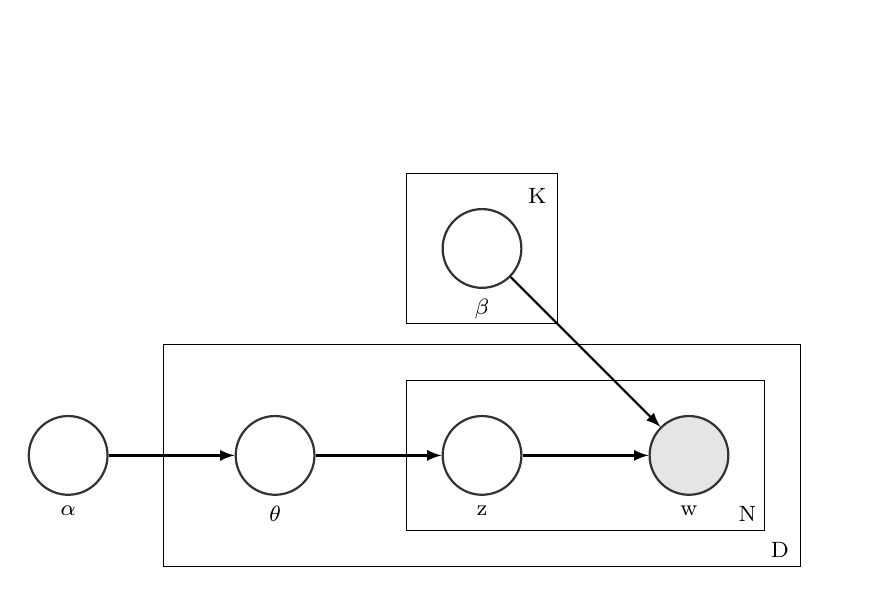
\begin{tikzpicture}
\tikzstyle{main}=[circle, minimum size = 10mm, thick, draw =black!80, node distance = 16mm]
\tikzstyle{connect}=[-latex, thick]
\tikzstyle{box}=[rectangle, draw=black!100]
  % sigma
  \node[main] (alpha) [label=below:$\alpha$] { };    
  % eta
  \node[main] (theta) [right=of alpha,label=below:$\theta$] { };
  % z
  \node[main] (z) [right=of theta,label=below:z] {};
  % beta
  \node[main] (beta) [above=of z,label=below:$\beta$] { };
%  \node[main] (beta) [left=of psi,label=below:$\beta$] { };
  \node[main, fill = black!10] (w) [right=of z,label=below:w] { };
  \path (alpha) edge [connect] (theta)
        (theta) edge [connect] (z)
		(z) edge [connect] (w)
		(beta) edge [connect] (w);
%		(beta) edge [connect] (psi);
  \node[rectangle, inner sep=4.4mm,draw=black!100, fit= (beta)] {};
  \node[rectangle, inner sep=4.4mm, fit= (beta), label=below right:K, xshift=-5mm, yshift=18.5mm] {};
  \node[rectangle, inner sep=0mm, fit= (z) (w),label=below right:N, , xshift=13mm] {};
  \node[rectangle, inner sep=4.4mm,draw=black!100, fit= (z) (w)] {};
    \node[rectangle, inner sep=4.6mm, fit= (z) (w),label=below right:D, xshift=12.5mm] {};
  \node[rectangle, inner sep=9mm, draw=black!100, fit = (theta) (z) (w)] {};
\end{tikzpicture}
\caption{Graphical representation for LDA}
\label{graph:lda}
\end{figure}
The mathematical formulation for LDA as follows.
\begin{itemize}
\item Joint Distribution for LDA
\begin{equation*}
\prod_{i=1}^{K}p(\beta_i)\left[\prod_{d=1}^{D}p(\theta_d)\prod_{n=1}^{N}p(z_{d,n}|\theta_d)p(w_{d,n}|\beta_{1:K},z_{d,n})\right]
\end{equation*} 
\item conditioning on $w_{1:D}$
\begin{equation*}
p(\beta_{1:K},\theta_{1:D},z_{1:D}|w_{1:D})=\frac{p(\beta_{1:K},\theta_{1:D},z_{1:D},w_{1:D})}{p(w_{1:D})}
\end{equation*}
\end{itemize}
\begin{algorithm}[H]
Initialize hyperparameters $ \alpha $, $ \beta $\\
\For{topic k in K}{
Sample a word distribution $ \phi_k\sim \text{Dir}(\beta) $
}
\For{document d in D}{
Sample a topic distribution $ \theta_d\sim \text{Dir}(\alpha) $\\
\For{word position n in $ N_d $}{
Sample a topic assignment $ z_{dn}\sim \text{Cat}(\theta_d) $\\
Sample a word $ w_{dn}\sim \text{Cat}(\phi_{z_{dn}}) $
}
}
\caption{Generative Process for LDA}
\end{algorithm}
The procedure for LDA as follows. For each topic k$\in$\{1,...,K\}, draw a multinomial distribution $\beta_k$ from a Dirichlet distribution with parameter $\lambda$. For each document d$\in$\{1,...,M\}, draw a multinomial distribution $\theta_d$ from a Dirichlet distribution with parameter $\alpha$. For each word position n$\in$\{1,...,N\}, select a topic $z_n$ from the Multinomial distribution parameterized by $\theta_d$. Choose the observed word $w_n$ from the distribution $\theta_{z_n}$.

%-------------------
\end{document}
the 